\chapter{内点法}
\label{chap:nonlinear-interior-point}

第~\ref{chap:lp-interior-point}章解线性规划时，从可行域内部沿中心路径走向最优解。那里的约束只是$x_i\geq0$，迭代点离每面墙有多远，看坐标就知道。现在换一个问题：在抛物线$x_2\geq x_1^2$与直线$x_2\leq4$围成的区域里，求离点$(3,0)$最近的点。墙是弯的，走一步之后，点离墙有多远要重新计算约束函数才知道。

路径跟踪的骨架可以保留：在边界上立起障碍，放宽互补条件，用Newton法沿参数曲线前进。需要重新回答的问题集中在四处。约束的曲率会进入线性方程组，Newton步可能不再是下降方向。严格内点不再一眼可见，乘子的符号也要专门维护。一个残差很小的点，未必满足原问题的最优性条件。更根本的是，线性规划有多项式时间的保证，一般光滑约束问题没有。

本章只讲这些新增的内容，线性规划里已经讲过的路径跟踪细节直接引用。第一节构造一般约束的障碍子问题，研究路径的存在性和间隙。第二节把松弛变量和乘子纳入同一组方程，推导Newton方向，并讨论步长的接受。第三节回答起点从哪里来、什么时候可以停。第四节把障碍换成二阶锥和半正定锥的形式。第五节说明哪些结论是全局证书，哪些只是局部结果，并计算每一轮的代价。

\section{障碍问题}
\label{sec:nlipm-barrier}

约束是一般的光滑函数时，怎样把“不许越界”写进目标，又让解最终能落到边界上？做法是求解一族带参数的内点子问题，再逐步减小参数。

\paragraph{问题与贯穿例}
本章讨论光滑约束问题
\begin{equation}
 \min_{\bm{x}\in\mathbb{R}^n}\ f(\bm{x})\quad\text{s.t.}\quad g_i(\bm{x})\leq0\ (i=1,\ldots,m),\quad h_j(\bm{x})=0\ (j=1,\ldots,p),
 \label{eq:nlipm-problem}
\end{equation}
其中$f$、$g_i$、$h_j$二阶连续可微。把约束值排成向量$\bm{g}(\bm{x})$、$\bm{h}(\bm{x})$，把它们的梯度按行排成两个Jacobian矩阵：
\begin{equation}
 \bm{J}(\bm{x})=\begin{bmatrix}\nabla g_1(\bm{x})^\top\\\vdots\\\nabla g_m(\bm{x})^\top\end{bmatrix}\in\mathbb{R}^{m\times n},\qquad
 \bm{A}(\bm{x})=\begin{bmatrix}\nabla h_1(\bm{x})^\top\\\vdots\\\nabla h_p(\bm{x})^\top\end{bmatrix}\in\mathbb{R}^{p\times n}.
 \label{eq:nlipm-jacobians}
\end{equation}
本章的$\bm{g}$始终表示约束值，不表示目标的梯度；目标梯度写成$\nabla f$。

全章贯穿下面这个二维例子：
\begin{equation}
 \begin{aligned}
 \min_{\bm{x}}\quad&f(\bm{x})=\tfrac12\bigl((x_1-3)^2+x_2^2\bigr)\\
 \text{s.t.}\quad&g_1(\bm{x})=x_1^2-x_2\leq0,\\
 &g_2(\bm{x})=x_2-4\leq0.
 \end{aligned}
 \label{eq:nlipm-running}
\end{equation}
可行集是抛物线之上、直线$x_2=4$之下的区域，目标是到点$\bm{c}=(3,0)^\top$的距离平方的一半。$g_1$是弯的约束，$g_2$是线性约束。

第~\ref{chap:constrained-optimality}章的KKT条件用到Lagrange函数
\begin{equation}
 \mathcal{L}(\bm{x},\bm{\lambda},\bm{\nu})=f(\bm{x})+\bm{\lambda}^\top\bm{g}(\bm{x})+\bm{\nu}^\top\bm{h}(\bm{x}).
 \label{eq:nlipm-lagrangian}
\end{equation}
条件是说：可行点$\bm{x}^\star$处存在乘子$\bm{\lambda}^\star\geq\bm{0}$和$\bm{\nu}^\star$，使$\mathcal{L}$对$\bm{x}$的梯度为零，并且$\lambda_i^\star g_i(\bm{x}^\star)=0$。

例~\eqref{eq:nlipm-running}中取$\bm{x}^\star=(1,1)^\top$，这时两个约束值和三个梯度是
\[
 g_1=0,\quad g_2=-3,\quad\nabla f=\begin{bmatrix}-2\\1\end{bmatrix},\quad\nabla g_1=\begin{bmatrix}2\\-1\end{bmatrix},\quad\nabla g_2=\begin{bmatrix}0\\1\end{bmatrix}.
\]
于是$\bm{\lambda}^\star=(1,0)^\top$满足全部KKT条件，最优值$f^\star=5/2$。问题是凸的，$\bm{x}^\star$就是全局解。图~\ref{fig:nlipm-running}画出了这一几何关系。

\begin{BookInlineFigure}
  \centering
  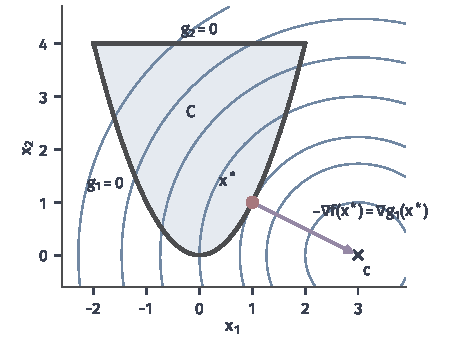
\includegraphics[width=76mm]{figures/05-optimization/06-constrained-optimization/matplotlib/nlipm-running/figure.pdf}
  \caption{贯穿例~\eqref{eq:nlipm-running}。浅蓝区域是可行集$\bm{C}$，深灰粗线是两段边界，蓝线是目标的等值线（以黑叉$\bm{c}=(3,0)$为圆心的圆），红点是最优解$\bm{x}^\star=(1,1)$。紫色箭头同时是$-\nabla f(\bm{x}^\star)$和$\nabla g_1(\bm{x}^\star)$，两者相等对应乘子$\lambda_1^\star=1$；直线边界不活动，乘子为零。}
  \label{fig:nlipm-running}
\end{BookInlineFigure}

\paragraph{内部只对不等式而言}
障碍只能加给不等式，因为只有不等式才有“里面”。记严格可行点的集合为
\begin{equation}
 \bm{C}^{\circ}=\bigl\{\bm{x}:g_i(\bm{x})<0\ (i=1,\ldots,m),\ \bm{h}(\bm{x})=\bm{0}\bigr\}.
 \label{eq:nlipm-strict-set}
\end{equation}
等式约束的可行点构成一张薄片，薄片上没有“离边界远一点”的余地。把$h=0$拆成$h\leq0$和$-h\leq0$也行不通，这两条不等式不可能同时严格成立，拆完之后$\bm{C}^{\circ}$是空集。所以等式约束继续显式保留，加上障碍之后的问题仍然是约束问题，而不是无约束问题。

\subsection{对数障碍}
\label{sec:nlipm-log-barrier}

第~\ref{chap:lp-interior-point}章对$x_i\geq0$用的障碍是$-\log x_i$。约束$x_i\geq0$也可以写成$g_i(\bm{x})=-x_i\leq0$，于是$-\log x_i=-\log(-g_i(\bm{x}))$。这个写法可以直接推广到任何$g_i$。

\begin{definition}[对数障碍函数]
\label{def:nlipm-barrier}
设$\bm{C}^{\circ}$非空。对$\mu>0$，$\bm{g}(\bm{x})<\bm{0}$的点上定义
\begin{equation}
 \phi(\bm{x})=-\sum_{i=1}^m\log\bigl(-g_i(\bm{x})\bigr),\qquad
 B_\mu(\bm{x})=f(\bm{x})+\mu\,\phi(\bm{x}).
 \label{eq:nlipm-barrier-function}
\end{equation}
相应的\term{障碍子问题}（barrier subproblem）是
\begin{equation}
 \min_{\bm{x}}\ B_\mu(\bm{x})\quad\text{s.t.}\quad\bm{h}(\bm{x})=\bm{0},\quad\bm{g}(\bm{x})<\bm{0}.
 \label{eq:nlipm-barrier-problem}
\end{equation}
\end{definition}

点靠近某条约束的边界时，$-g_i\downarrow0$，$\phi\to+\infty$。边界像一堵墙，迭代点靠函数值的上升留在内部。例~\eqref{eq:nlipm-running}的障碍目标是
\[
 B_\mu(\bm{x})=\tfrac12\bigl((x_1-3)^2+x_2^2\bigr)-\mu\log(x_2-x_1^2)-\mu\log(4-x_2).
\]
图~\ref{fig:nlipm-barrier-bowls}画出两个参数下的等值线。参数较大时碗底靠近区域中央，参数较小时等值线贴向边界，碗底被目标拉向$\bm{x}^\star$。

\begin{BookInlineFigure}
  \centering
  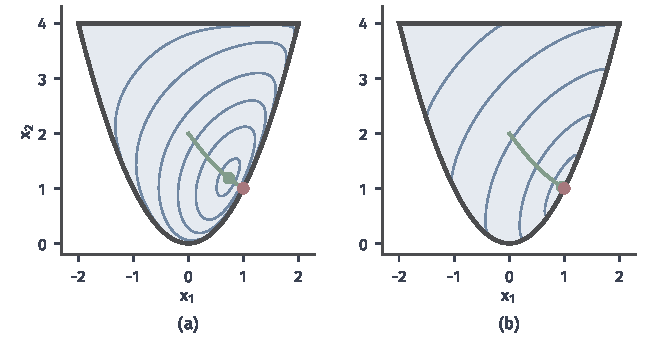
\includegraphics[width=112mm]{figures/05-optimization/06-constrained-optimization/matplotlib/nlipm-barrier-bowls/figure.pdf}
  \caption{贯穿例的障碍目标$B_\mu$在可行集内的等值线（蓝线）。(a)$\mu=1$；(b)$\mu=0.1$。绿线是各参数下碗底连成的曲线，绿点是当前参数的碗底，红点是$\bm{x}^\star$。}
  \label{fig:nlipm-barrier-bowls}
\end{BookInlineFigure}

\paragraph{约束的梯度和Hessian怎样进入}
求导只需要复合函数法则。对一元函数$\psi(u)=-\log(-u)$（$u<0$），有
\[
 \psi'(u)=\frac{1}{-u},\qquad\psi''(u)=\frac{1}{u^2}.
\]
把$u=g_i(\bm{x})$代入，并对$i$求和，得到障碍函数的梯度和Hessian：
\begin{align}
 \nabla\phi(\bm{x})&=\sum_{i=1}^m\frac{1}{-g_i(\bm{x})}\,\nabla g_i(\bm{x}),
 \label{eq:nlipm-barrier-grad}\\
 \nabla^2\phi(\bm{x})&=\sum_{i=1}^m\frac{\nabla g_i(\bm{x})\nabla g_i(\bm{x})^\top}{g_i(\bm{x})^2}
 +\sum_{i=1}^m\frac{\nabla^2g_i(\bm{x})}{-g_i(\bm{x})}.
 \label{eq:nlipm-barrier-hess}
\end{align}

式~\eqref{eq:nlipm-barrier-hess}的两项作用不同。第一项是秩一矩阵之和，只在约束的法向产生曲率，点越靠近边界越大，这就是“墙”的刚度。第二项把约束本身的弯曲带进来，线性规划中$\nabla^2g_i=\bm{0}$，这一项不存在，所以它正是本章新增的内容。

在贯穿例的点$\bm{x}=(1,2)^\top$上算一次。约束值与约束梯度是
\[
 g_1=-1,\quad g_2=-2,\quad\nabla g_1=\begin{bmatrix}2\\-1\end{bmatrix},\quad\nabla g_2=\begin{bmatrix}0\\1\end{bmatrix},\quad\nabla^2g_1=\begin{bmatrix}2&0\\0&0\end{bmatrix}.
\]
代入式~\eqref{eq:nlipm-barrier-grad}，得到
\[
 \nabla\phi=1\cdot\begin{bmatrix}2\\-1\end{bmatrix}+\frac12\begin{bmatrix}0\\1\end{bmatrix}=\begin{bmatrix}2\\-1/2\end{bmatrix}.
\]
代入式~\eqref{eq:nlipm-barrier-hess}，三块矩阵相加：
\[
 \nabla^2\phi=\begin{bmatrix}4&-2\\-2&1\end{bmatrix}+\begin{bmatrix}0&0\\0&1/4\end{bmatrix}+\begin{bmatrix}2&0\\0&0\end{bmatrix}=\begin{bmatrix}6&-2\\-2&5/4\end{bmatrix}.
\]
最后一块$\operatorname{diag}(2,0)$来自抛物线的弯曲，如果把$g_1$换成切线，它就消失了。

\paragraph{一维边界例子：内点步受到的限制}
Newton法用二次模型近似$B_\mu$，而障碍函数在边界附近根本不像二次函数。看最简单的弯约束：
\[
 \min_x\ x\quad\text{s.t.}\quad x^2-1\leq0.
\]
解是$x^\star=-1$。障碍目标$B_\mu(x)=x-\mu\log(1-x^2)$的导数是
\[
 B_\mu'(x)=1+\frac{2\mu x}{1-x^2},\qquad B_\mu''(x)=\frac{2\mu(1+x^2)}{(1-x^2)^2}.
\]
令$B_\mu'(x)=0$，得到$1-x^2+2\mu x=0$。在$(-1,1)$内的根是
\begin{equation}
 x(\mu)=\mu-\sqrt{\mu^2+1}.
 \label{eq:nlipm-1d-center}
\end{equation}
取几个能算成分数的值：$\mu=3/4$时$x=-1/2$，$\mu=5/12$时$x=-2/3$。

现在站在$\mu=3/4$的碗底$x=-1/2$，把参数减小到$\mu^+$，走一个Newton步。在这一点上
\[
 \frac{2x}{1-x^2}=-\frac43,\qquad\frac{2(1+x^2)}{(1-x^2)^2}=\frac{40}{9}.
\]
于是Newton步是
\[
 d=-\frac{1-\tfrac43\mu^+}{\tfrac{40}{9}\mu^+}=-\frac{9-12\mu^+}{40\mu^+}.
\]

$\mu^+=5/12$时$d=-6/25$，新点$-0.74$仍在区间内，离新的碗底$-2/3$不远。$\mu^+=0.05$时$d=-4.2$，新点是$-4.7$，已经远在可行域之外，如图~\ref{fig:nlipm-barrier-1d}(b)所示。要让单位步留在区间内，需要$d>-1/2$，解这个不等式，得到
\[
 \mu^+>\frac{9}{32}.
\]
也就是说，这一点上参数最多缩小到原来的$3/8$。参数一次减得太多，碗底搬走了，二次模型却还停留在旧的位置。

\begin{BookInlineFigure}
  \centering
  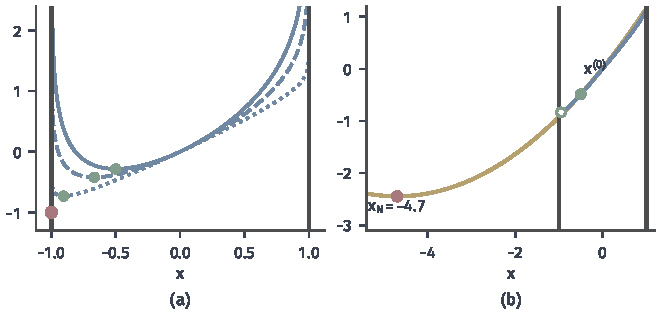
\includegraphics[width=112mm]{figures/05-optimization/06-constrained-optimization/matplotlib/nlipm-barrier-1d/figure.pdf}
  \caption{一维边界例子$\min x$，$x^2\leq1$。(a)蓝线是$B_\mu$，实线、虚线、点线分别对应$\mu=3/4$、$5/12$、$0.1$，绿点是碗底，红点是解$x^\star=-1$，深灰粗线是边界$x=\pm1$。(b)参数减到$\mu^+=0.05$，蓝线是$B_{\mu^+}$，只在区间内有定义；黄线是在绿点$x^{(0)}=-1/2$处的二次模型，其极小点（红点）落在$-4.7$；空心绿点是新的碗底。}
  \label{fig:nlipm-barrier-1d}
\end{BookInlineFigure}

\paragraph{新的曲率与凸性}
约束的弯曲方向决定第二项的符号。$g_i$凸时$\nabla^2g_i\succeq\bm{0}$，第二项半正定，障碍函数保持凸性。

\begin{lemma}[凸约束的障碍是凸函数]
\label{lem:nlipm-barrier-convex}
设每个$g_i$在开集上凸且二阶连续可微，则$\phi$在集合$\{\bm{x}:\bm{g}(\bm{x})<\bm{0}\}$的每个凸子集上是凸函数。
\end{lemma}

\begin{proof}
式~\eqref{eq:nlipm-barrier-hess}中，第一项是半正定矩阵的非负组合。第二项中$-g_i>0$，$\nabla^2g_i\succeq\bm{0}$，也是半正定矩阵的非负组合。所以$\nabla^2\phi\succeq\bm{0}$。
\end{proof}

$g_i$非凸时，这个结论没有理由成立，用了对数也不会自动得到凸子问题。看单位圆盘的外部，约束是$g(\bm{x})=1-\lVert\bm{x}\rVert_2^2\leq0$。这时$\nabla^2g=-2\bm{I}$，式~\eqref{eq:nlipm-barrier-hess}给出
\[
 \nabla^2\phi(\bm{x})=\frac{4\bm{x}\bm{x}^\top}{(\lVert\bm{x}\rVert_2^2-1)^2}-\frac{2\bm{I}}{\lVert\bm{x}\rVert_2^2-1}.
\]
沿与$\bm{x}$垂直的切向，第一项为零，第二项是负的，曲率等于$-2/(\lVert\bm{x}\rVert_2^2-1)$，离边界越近越负。

图~\ref{fig:nlipm-nonconvex-barrier}取目标$x_2^2+0.12(x_1-1/2)^2$，并取$\mu=0.1$。障碍目标有两个彼此隔开的局部极小点，分别在圆盘的右侧和左侧。图(b)沿点$(1.5,0)$处的切向对比两种约束：外部约束的障碍在这一点是山顶形状，圆盘内部约束的障碍则是碗。

\begin{BookInlineFigure}
  \centering
  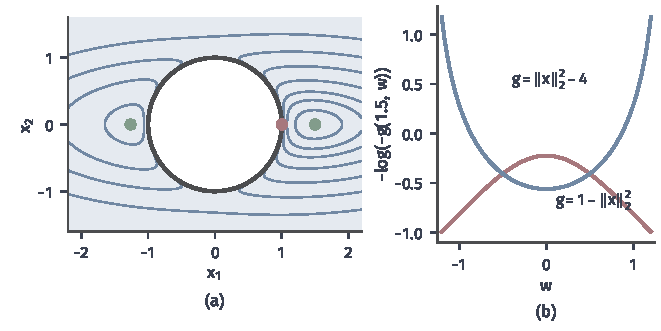
\includegraphics[width=112mm]{figures/05-optimization/06-constrained-optimization/matplotlib/nlipm-nonconvex-barrier/figure.pdf}
  \caption{非凸约束的障碍。(a)可行集是单位圆盘的外部（浅蓝），蓝线是$B_{0.1}$的等值线，两个绿点是障碍目标的局部极小点，红点是原问题的全局解$(1,0)$。(b)沿$x_1=1.5$的切向，红线是外部约束$g=1-\lVert\bm{x}\rVert_2^2$的障碍，在$w=0$处曲率为负；蓝线是圆盘内部约束$g=\lVert\bm{x}\rVert_2^2-4$的障碍，曲率为正。}
  \label{fig:nlipm-nonconvex-barrier}
\end{BookInlineFigure}

\subsection{参数与路径}
\label{sec:nlipm-parameter-path}

固定一个$\mu$，子问题~\eqref{eq:nlipm-barrier-problem}有没有解？解随$\mu$怎样变？这一小节先用驻定条件把子问题和KKT条件联系起来，再分凸问题和非凸问题回答这两个问题。

\paragraph{驻定条件就是扰动的互补}
子问题~\eqref{eq:nlipm-barrier-problem}的一阶条件是：存在$\bm{\nu}$，使
\[
 \nabla B_\mu(\bm{x})+\bm{A}(\bm{x})^\top\bm{\nu}=\bm{0}.
\]
把式~\eqref{eq:nlipm-barrier-grad}代入，得到
\[
 \nabla f(\bm{x})+\sum_{i=1}^m\frac{\mu}{-g_i(\bm{x})}\nabla g_i(\bm{x})+\bm{A}(\bm{x})^\top\bm{\nu}=\bm{0}.
\]

求和中的系数都是正数，并且正好处在KKT条件中乘子的位置。令$\lambda_i=\mu/(-g_i(\bm{x}))$，条件变成
\begin{equation}
 \begin{gathered}
 \nabla f(\bm{x})+\bm{J}(\bm{x})^\top\bm{\lambda}+\bm{A}(\bm{x})^\top\bm{\nu}=\bm{0},\qquad\bm{h}(\bm{x})=\bm{0},\\
 \lambda_i\bigl(-g_i(\bm{x})\bigr)=\mu\ (i=1,\ldots,m),\qquad\bm{g}(\bm{x})<\bm{0},\quad\bm{\lambda}>\bm{0}.
 \end{gathered}
 \label{eq:nlipm-perturbed-kkt}
\end{equation}
与KKT条件逐项比较，只有互补一处不同：$\lambda_ig_i=0$换成了$\lambda_i(-g_i)=\mu$。这和第~\ref{chap:lp-interior-point}章的$x_is_i=\mu$是同一件事。乘子不是另外猜出来的，它就是障碍项在该约束上施加的推力，$\lambda_i=\mu/(-g_i)$离墙越近越大。

\paragraph{子问题的解何时存在}
碗底的存在要靠水平集被围住。下面的定理说明，可行集有界时墙就足够了。

\begin{theorem}[障碍子问题的解]
\label{thm:nlipm-barrier-exists}
设$f$、$g_i$、$h_j$连续，可行集$\bm{C}$有界，$\bm{C}^{\circ}$非空，$\mu>0$。则$B_\mu$在$\bm{C}^{\circ}$上取到最小值。

再设$f$、$g_i$凸且二阶连续可微，$\bm{h}(\bm{x})=\bm{A}\bm{x}-\bm{b}$，$\bm{A}$满行秩，并且不存在非零的$\bm{d}$同时满足
\begin{equation}
 \bm{A}\bm{d}=\bm{0},\quad\bm{d}^\top\nabla^2f\bm{d}=0,\quad\nabla g_i^\top\bm{d}=0,\quad\bm{d}^\top\nabla^2g_i\bm{d}=0\ (\forall i)
 \label{eq:nlipm-unique-condition}
\end{equation}
（各导数在$\bm{C}^{\circ}$的任一点取值）。则最小点$\bm{x}(\mu)$唯一，方程组~\eqref{eq:nlipm-perturbed-kkt}有唯一解$(\bm{x}(\mu),\bm{\lambda}(\mu),\bm{\nu}(\mu))$。
\end{theorem}

\begin{proof}
先证存在。$\bm{C}$是有界闭集，$f$和每个$-g_i$在其上连续，所以存在常数$F$和$G>1$，使$\lvert f\rvert\leq F$，$-g_i\leq G$。

取$\bm{x}^{(0)}\in\bm{C}^{\circ}$，考虑下水平集
\[
 \bigl\{\bm{x}\in\bm{C}^{\circ}:B_\mu(\bm{x})\leq B_\mu(\bm{x}^{(0)})\bigr\}.
\]
对其中的点和任一下标$i$，把其余各项移到右边，得到
\[
 -\mu\log\bigl(-g_i(\bm{x})\bigr)\leq B_\mu(\bm{x}^{(0)})+F+\mu(m-1)\log G.
\]
右端是常数，所以存在$\epsilon>0$，使$-g_i(\bm{x})\geq\epsilon$。这说明水平集是$\bm{C}$的闭子集，从而是紧集，连续函数$B_\mu$在其上取到最小值。

再证唯一。由引理~\ref{lem:nlipm-barrier-convex}，$B_\mu$凸。对满足$\bm{A}\bm{d}=\bm{0}$的非零$\bm{d}$，式~\eqref{eq:nlipm-barrier-hess}给出
\[
 \bm{d}^\top\nabla^2B_\mu\bm{d}=\bm{d}^\top\nabla^2f\bm{d}+\mu\sum_{i=1}^m\Bigl(\frac{(\nabla g_i^\top\bm{d})^2}{g_i^2}+\frac{\bm{d}^\top\nabla^2g_i\bm{d}}{-g_i}\Bigr).
\]
右端各项非负，由条件~\eqref{eq:nlipm-unique-condition}，它们不全为零，所以$B_\mu$在仿射集上严格凸，最小点唯一。

最后看方程组。最小点处梯度与$\bm{A}$的零空间正交，所以存在$\bm{\nu}$使驻定条件成立，$\bm{A}$满行秩使$\bm{\nu}$唯一，$\bm{\lambda}$由$\lambda_i=\mu/(-g_i)$确定。反过来，方程组的解满足凸函数$B_\mu$在仿射集上的一阶条件，因此就是最小点。
\end{proof}

存在性的第一部分没有用到凸性，它只用到有界和连续。可行集无界时，这个结论可能失败。问题$\min 0$、$-x\leq0$的最优解集是$[0,\infty)$，障碍目标$-\mu\log x$在$x\to\infty$时趋于$-\infty$，没有最小点。条件~\eqref{eq:nlipm-unique-condition}在贯穿例中成立，因为$\nabla^2f=\bm{I}$，第二项已经排除了所有非零方向。

\paragraph{路径}
定理的条件成立时，$\mu$取遍$(0,\infty)$，解连成一条曲线，沿用第~\ref{chap:lp-interior-point}章的名字，称为中心路径。图~\ref{fig:nlipm-central-path}画出贯穿例的路径。当$\mu\to\infty$时，目标的作用可以忽略，点趋于$\phi$的最小点，即解析中心。贯穿例的解析中心可以直接求：对称性给出$x_1=0$，再由$-1/x_2+1/(4-x_2)=0$得到$x_2=2$。

\begin{BookInlineFigure}
  \centering
  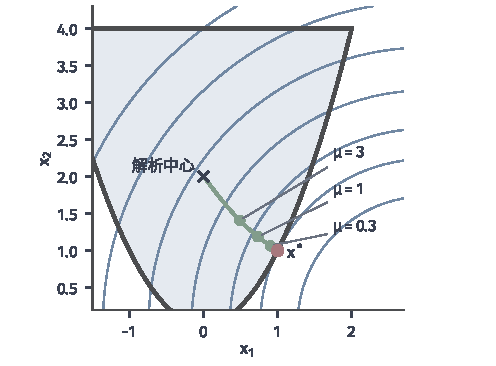
\includegraphics[width=84mm]{figures/05-optimization/06-constrained-optimization/matplotlib/nlipm-central-path/figure.pdf}
  \caption{贯穿例的中心路径（绿线）。黑叉是解析中心$(0,2)$，绿点是$\mu=3$、$1$、$0.3$对应的中心点，红点是$\bm{x}^\star=(1,1)$，蓝线是目标的等值线。路径是弯的，因为不活动的直线约束的影响在逐渐消失。}
  \label{fig:nlipm-central-path}
\end{BookInlineFigure}

这个例子的路径可以化成一元方程。由方程组~\eqref{eq:nlipm-perturbed-kkt}的第一行，$\lambda_1=(3-x_1)/(2x_1)$。取$\mu=1$，用Newton法解出的中心点和乘子是
\[
 \bm{x}(1)\approx(0.7343,1.1873)^\top,\qquad\bm{\lambda}(1)\approx(1.5428,0.3555)^\top.
\]
可以核对互补：$\lambda_1(x_2-x_1^2)=1.5428\times0.6481\approx1$，$\lambda_2(4-x_2)=0.3555\times2.8127\approx1$。

图~\ref{fig:nlipm-path-multipliers}(a)显示乘子沿路径的走向。活动约束的乘子$\lambda_1(\mu)$趋于$\lambda_1^\star=1$，不活动约束的乘子$\lambda_2(\mu)$按$\mu/3$的量级趋于零，这里的$3$就是直线约束在解处的松弛。乘子估计本身就在告诉我们哪条约束活动，这一点不需要事先猜测。

\paragraph{凸问题的间隙}
第~\ref{chap:lp-interior-point}章中，沿路径的对偶间隙恰好是$n\mu$。一般凸问题也有同样的结果，只是$n$要换成不等式的条数$m$。

\begin{theorem}[路径上的间隙]
\label{thm:nlipm-gap}
设$f$、$g_i$凸且可微，$\bm{h}(\bm{x})=\bm{A}\bm{x}-\bm{b}$，$(\bm{x},\bm{\lambda},\bm{\nu})$满足方程组~\eqref{eq:nlipm-perturbed-kkt}，$f^\star$是问题~\eqref{eq:nlipm-problem}在可行集上的下确界。则
\begin{equation}
 f(\bm{x})-m\mu\leq f^\star\leq f(\bm{x}).
 \label{eq:nlipm-gap}
\end{equation}
\end{theorem}

\begin{proof}
右边的不等式成立是因为$\bm{x}$可行。对左边，任取可行点$\bm{x}'$。因为$\bm{\lambda}>\bm{0}$、$\bm{g}(\bm{x}')\leq\bm{0}$、$\bm{h}(\bm{x}')=\bm{0}$，有
\[
 f(\bm{x}')\geq f(\bm{x}')+\bm{\lambda}^\top\bm{g}(\bm{x}')+\bm{\nu}^\top\bm{h}(\bm{x}')=\mathcal{L}(\bm{x}',\bm{\lambda},\bm{\nu}).
\]

$\mathcal{L}(\cdot,\bm{\lambda},\bm{\nu})$是凸函数，并且在$\bm{x}$处梯度为零，所以$\bm{x}$是它的全局最小点：
\[
 \mathcal{L}(\bm{x}',\bm{\lambda},\bm{\nu})\geq\mathcal{L}(\bm{x},\bm{\lambda},\bm{\nu}).
\]

再用$\bm{h}(\bm{x})=\bm{0}$和$\lambda_ig_i(\bm{x})=-\mu$，得到
\[
 \mathcal{L}(\bm{x},\bm{\lambda},\bm{\nu})=f(\bm{x})+\sum_{i=1}^m\lambda_ig_i(\bm{x})=f(\bm{x})-m\mu.
\]
三式相连，对$\bm{x}'$取下确界即得。
\end{proof}

式~\eqref{eq:nlipm-gap}的左端是一个对偶值，它由当前点直接算出，不需要知道$\bm{x}^\star$。要保证目标误差不超过$\varepsilon$，走到$\mu\leq\varepsilon/m$就够了。

这个界数的是全部$m$条约束，实际误差往往更小。图~\ref{fig:nlipm-path-multipliers}(b)中，贯穿例的$f(\bm{x}(\mu))-f^\star$在$\mu$小时约等于$\mu$，而不是$2\mu$。原因是不活动的约束虽然也贡献了$\lambda_2s_2=\mu$，它却只是把对偶值往下拉，并不代表目标还有这么多可以下降。

\begin{BookInlineFigure}
  \centering
  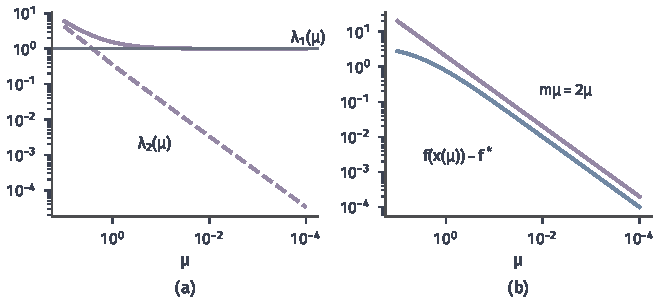
\includegraphics[width=112mm]{figures/05-optimization/06-constrained-optimization/matplotlib/nlipm-path-multipliers/figure.pdf}
  \caption{贯穿例沿中心路径的量，横轴是$\mu$，向右减小。(a)紫色实线是$\lambda_1(\mu)$，趋于$\lambda_1^\star=1$（灰线）；紫色虚线是$\lambda_2(\mu)$，随$\mu$线性趋于零。(b)紫线是定理的界$m\mu=2\mu$，蓝线是实际误差$f(\bm{x}(\mu))-f^\star$。}
  \label{fig:nlipm-path-multipliers}
\end{BookInlineFigure}

\paragraph{固定参数时解多准，参数降多快}
这样就得到\term{障碍法}（barrier method）：外层维护参数$\mu$，内层从上一个点出发，用第~\ref{chap:second-order-methods}章的阻尼Newton法解子问题~\eqref{eq:nlipm-barrier-problem}，解到Newton减量足够小，再令$\mu\leftarrow\tau\mu$，其中$\tau\in(0,1)$。回溯时要多加一条规则，试探点若使某个$g_i\geq0$，直接拒绝。

以贯穿例从$\bm{x}^{(0)}=(1,2)^\top$、$\mu=1$开始。前面已经算出$\nabla\phi$和$\nabla^2\phi$，把目标的导数加上，得到
\[
 \nabla B_1=\begin{bmatrix}0\\3/2\end{bmatrix},\qquad\nabla^2B_1=\begin{bmatrix}7&-2\\-2&9/4\end{bmatrix}.
\]
解线性方程组，Newton方向是
\[
 \bm{d}=\Bigl(-\frac{12}{47},\,-\frac{42}{47}\Bigr)^\top\approx(-0.2553,\,-0.8936)^\top.
\]
单位步后的点$(0.7447,1.1064)^\top$仍然严格可行，再走两步就到达$\bm{x}(1)$附近。

外层有两种取舍。$\tau$接近$1$时，上一个点几乎就是新碗底，每轮只需一两个Newton步，但要走很多轮。$\tau$很小时，轮数少，但正如一维例子所示，起步时Newton步很不可靠，每轮要靠回溯慢慢走。

图~\ref{fig:nlipm-update-tradeoff}是贯穿例上的实测，从解析中心出发，要求$m\mu\leq10^{-6}$。$\tau=0.9$时总共要$218$个Newton步，$\tau=0.5$时$38$步，$\tau=0.1$时$32$步，$\tau=0.001$时只要$18$步，单轮最多也不过$6$步。这说明Newton步的总数对$\tau$不敏感，只有$\tau$过于接近$1$时明显吃亏。

这是一个二维小例子上的观察，并且总数随$\tau$并不单调。规模增大时，大幅度减小参数的代价一般会更明显，第~\ref{sec:nlipm-guarantees}节再谈理论上的界。

\begin{BookInlineFigure}
  \centering
  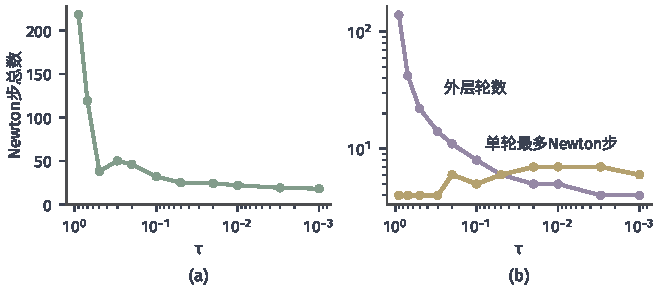
\includegraphics[width=112mm]{figures/05-optimization/06-constrained-optimization/matplotlib/nlipm-update-tradeoff/figure.pdf}
  \caption{贯穿例上障碍法的工作量，$\mu^{(0)}=1$，内层Newton减量阈值$10^{-8}$，横轴是参数缩小倍率$\tau$，向右更激进。(a)Newton步总数。(b)紫线是外层轮数，黄线是单轮最多的Newton步数。}
  \label{fig:nlipm-update-tradeoff}
\end{BookInlineFigure}

\paragraph{非凸问题只能谈局部路径}
没有凸性时，定理~\ref{thm:nlipm-gap}的推理在“$\bm{x}$是$\mathcal{L}$的全局最小点”这一步断掉，方程组~\eqref{eq:nlipm-perturbed-kkt}的解也不必唯一。能保证的是在一个性质好的KKT点附近，有一段路径通向它。

\begin{theorem}[KKT点附近的路径]
\label{thm:nlipm-local-path}
设$f$、$g_i$、$h_j$二阶连续可微，$(\bm{x}^\star,\bm{\lambda}^\star,\bm{\nu}^\star)$是KKT点，并满足三个条件：活动约束梯度与全部等式约束梯度线性无关；严格互补，即活动约束的乘子都为正；在临界方向上有
\begin{equation}
 \bm{d}^\top\nabla_{\bm{x}\bm{x}}^2\mathcal{L}(\bm{x}^\star,\bm{\lambda}^\star,\bm{\nu}^\star)\bm{d}>0,
 \label{eq:nlipm-sosc}
\end{equation}
这里临界方向指满足$\bm{A}\bm{d}=\bm{0}$、对活动约束$\nabla g_i^\top\bm{d}=0$的非零$\bm{d}$。则存在$\bar{\mu}>0$和连续可微的曲线$\mu\mapsto(\bm{x}(\mu),\bm{\lambda}(\mu),\bm{\nu}(\mu))$，在$(0,\bar{\mu})$上满足方程组~\eqref{eq:nlipm-perturbed-kkt}，$\mu\downarrow0$时趋于该KKT点，并且$\bm{x}(\mu)$是子问题~\eqref{eq:nlipm-barrier-problem}的严格局部极小点。
\end{theorem}

\begin{proof}
设$\bm{s}=-\bm{g}$，把方程组写成关于$(\bm{x},\bm{s},\bm{\lambda},\bm{\nu})$的方程$\bm{F}(\cdot)=\mu\bm{e}$，其中$\bm{e}$只在互补方程处为$1$。在$\mu=0$的KKT点处用隐函数定理，只需证明Jacobian矩阵非奇异，也就是下面的齐次方程只有零解：
\[
 \begin{gathered}
 \bm{W}\bm{d}+\bm{J}^\top\bm{d}_\lambda+\bm{A}^\top\bm{d}_\nu=\bm{0},\qquad\bm{A}\bm{d}=\bm{0},\\
 \bm{J}\bm{d}+\bm{d}_s=\bm{0},\qquad\lambda_i^\star d_{s,i}+s_i^\star d_{\lambda,i}=0.
 \end{gathered}
\]
这里$\bm{W}=\nabla^2_{\bm{x}\bm{x}}\mathcal{L}$。

对活动约束，$s_i^\star=0$、$\lambda_i^\star>0$，互补方程给出$d_{s,i}=0$，于是$\nabla g_i^\top\bm{d}=0$。对不活动约束，$\lambda_i^\star=0$、$s_i^\star>0$，互补方程给出$d_{\lambda,i}=0$。

用$\bm{d}^\top$左乘第一个方程，再用$\bm{A}\bm{d}=\bm{0}$，得到
\[
 \bm{d}^\top\bm{W}\bm{d}=-\sum_{i}d_{\lambda,i}\nabla g_i^\top\bm{d}=0.
\]
求和中每一项都为零：活动约束的$\nabla g_i^\top\bm{d}=0$，不活动约束的$d_{\lambda,i}=0$。由条件~\eqref{eq:nlipm-sosc}，$\bm{d}=\bm{0}$。

于是$\bm{d}_s=\bm{0}$，第一个方程只剩活动约束与等式约束的梯度组合等于零，由线性无关性，$\bm{d}_\lambda$、$\bm{d}_\nu$为零。隐函数定理给出连续可微的解曲线。对小的$\mu>0$，活动约束$s_i=\mu/\lambda_i>0$，不活动约束$\lambda_i=\mu/s_i>0$，所以解满足正性要求。

最后证局部极小。把式~\eqref{eq:nlipm-barrier-hess}和$\lambda_i=\mu/s_i$代入$\nabla^2B_\mu$，并计入等式约束的曲率，子问题的Lagrange Hessian是$\bm{W}+\bm{J}^\top\bm{S}^{-1}\bm{\Lambda}\bm{J}$，其中$\bm{S}$、$\bm{\Lambda}$是对角矩阵。假设存在$\mu_k\downarrow0$和单位向量$\bm{d}_k$，满足$\bm{A}\bm{d}_k=\bm{0}$，而二次型非正。则
\[
 \sum_{i}\frac{\lambda_i}{s_i}(\nabla g_i^\top\bm{d}_k)^2\leq-\bm{d}_k^\top\bm{W}\bm{d}_k.
\]
右端有界，而活动约束的$\lambda_i/s_i\to\infty$，所以极限方向$\bar{\bm{d}}$满足$\nabla g_i^\top\bar{\bm{d}}=0$。于是$\bar{\bm{d}}$是临界方向，并且$\bar{\bm{d}}^\top\bm{W}\bar{\bm{d}}\leq0$，与式~\eqref{eq:nlipm-sosc}矛盾。
\end{proof}

定理的三个条件各管一件事。线性无关保证乘子唯一，严格互补保证每条约束在极限时明确属于活动或不活动的一侧，式~\eqref{eq:nlipm-sosc}保证弯曲方向上是极小而不是鞍点。

隐函数定理还给出路径在$\mu=0$处的切线。在贯穿例中，$\bm{W}=\operatorname{diag}(3,1)$，$s_2^\star=3$，把解曲线对$\mu$求导，得到
\[
 \lambda_2'(0)=\frac13,\qquad s_1'(0)=1.
\]
线性化的方程剩下三个未知量$x_1'$、$x_2'$、$\lambda_1'$，解出
\[
 \bm{x}'(0)=\Bigl(-\frac{8}{21},\,\frac{5}{21}\Bigr)^\top,\qquad\lambda_1'(0)=\frac47.
\]
所以$\bm{x}(\mu)\approx(1,1)^\top+\mu(-8/21,5/21)^\top$。取$\mu=0.01$，预测$(0.9962,1.0024)^\top$，数值解是$(0.9962,1.0024)^\top$。目标的一阶变化是$\nabla f^\top\bm{x}'(0)=1$，这正是前面看到的“误差约等于$\mu$”。

\paragraph{路径可以断开，也可能通向较差的解}
定理~\ref{thm:nlipm-local-path}的$\bar{\mu}$可以很小，它不保证路径能一直延伸到大的$\mu$。下面的一维例子说明会发生什么。在$x>0$上取$f'(x)=(x-1)(x-3)(x-4)$，它在$x=1$和$x=4$处有局部极小，$f(4)-f(1)=9/4$，所以$x=1$是全局解。

障碍驻定条件$f'(x)=\mu/x$可以反解成
\[
 \mu=x(x-1)(x-3)(x-4).
\]
要求$\mu>0$，可行的$x$只有$(1,3)$和$(4,\infty)$两段。第一段上$\mu$先增后减，在$x=2$处达到最大值$\mu=4$。图~\ref{fig:nlipm-nonconvex-fold}(b)中，极小点的分支从$x=1$出发，到$\mu=4$时与鞍点分支相撞，两者同时消失，这个点称为\term{折叠点}（fold point）。

$\mu>4$时只剩$x>4$这一支。从大的$\mu$出发沿路径减小参数，走到的是$x=4$，错过了全局解$x=1$。这条路径是连续的，算法并没有失败，只是路径根本不经过全局解。

\begin{BookInlineFigure}
  \centering
  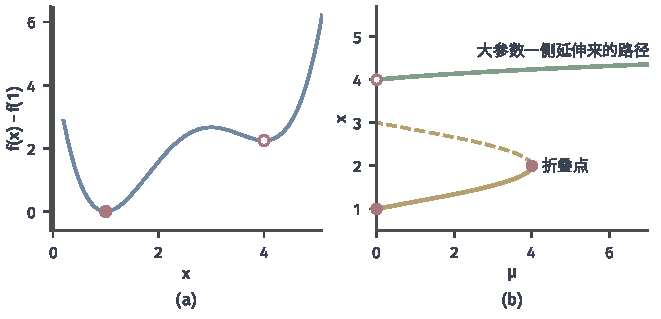
\includegraphics[width=112mm]{figures/05-optimization/06-constrained-optimization/matplotlib/nlipm-nonconvex-fold/figure.pdf}
  \caption{非凸的一维路径，$f'(x)=(x-1)(x-3)(x-4)$，$x>0$。(a)蓝线是目标，红点是全局解$x=1$，空心红点是局部解$x=4$。(b)$(\mu,x)$平面上的驻点集合：绿线是从大参数一侧延伸来的路径；黄线是$(1,3)$上的另一支，实线部分是局部极小点，虚线部分不是，两者在红点（折叠点$(4,2)$）相遇。}
  \label{fig:nlipm-nonconvex-fold}
\end{BookInlineFigure}

\section{原始—对偶内点法}
\label{sec:nlipm-primal-dual}

障碍法有两个不便之处。一维例子已经显示，参数减小之后，从旧碗底出发的Newton步可能完全不可信。另外它要求每个迭代点都严格满足$\bm{g}(\bm{x})<\bm{0}$，弯的约束使这件事代价不小。于是要问：把乘子和松弛都当作独立变量，同时更新，能否绕开这两点，又要付出什么代价？

\subsection{扰动互补方程}
\label{sec:nlipm-perturbed}

方程组~\eqref{eq:nlipm-perturbed-kkt}里，$-g_i$既是约束值，又是互补方程的一个因子。引入\term{松弛变量}（slack variable）$\bm{s}\in\mathbb{R}^m$，把它们分开：
\begin{equation}
 \begin{aligned}
 \nabla f(\bm{x})+\bm{J}(\bm{x})^\top\bm{\lambda}+\bm{A}(\bm{x})^\top\bm{\nu}&=\bm{0},\\
 \bm{h}(\bm{x})&=\bm{0},\\
 \bm{g}(\bm{x})+\bm{s}&=\bm{0},\\
 s_i\lambda_i&=\mu\quad(i=1,\ldots,m),\\
 \bm{s}>\bm{0},\quad\bm{\lambda}&>\bm{0}.
 \end{aligned}
 \label{eq:nlipm-pd-system}
\end{equation}
这里的乘子$\bm{\lambda}$沿用第~\ref{chap:constrained-optimality}章的符号。要留意$\bm{s}$的角色变了：第~\ref{chap:lp-interior-point}章的$\bm{s}$是对偶松弛，这里的$\bm{s}$是原始松弛，对偶一侧的正变量是$\bm{\lambda}$。表~\ref{tab:nlipm-lp-correspondence}列出两章量的对应，取$\bm{g}(\bm{x})=-\bm{x}$就回到线性规划。

\begin{BookInlineTable}
  \centering
  \footnotesize
  \begin{tabular}{@{}lll@{}}
    \toprule
    量 & 线性规划 & 一般约束\\
    \midrule
    原始侧的正变量 & $\bm{x}$ & $\bm{s}=-\bm{g}(\bm{x})$\\
    对偶侧的正变量 & $\bm{s}$ & $\bm{\lambda}$\\
    扰动互补 & $x_is_i=\mu$ & $s_i\lambda_i=\mu$\\
    不等式约束数 & $n$ & $m$\\
    Jacobian & $-\bm{I}$，常数 & $\bm{J}(\bm{x})$，随点变化\\
    等式的Jacobian & $\bm{A}$，常数 & $\bm{A}(\bm{x})$，随点变化\\
    二阶信息 & 无 & Lagrange Hessian\\
    \bottomrule
  \end{tabular}
  \caption{线性规划内点法与一般约束内点法中各量的对应。}
  \label{tab:nlipm-lp-correspondence}
\end{BookInlineTable}

\paragraph{正性和参数各管什么}
方程组~\eqref{eq:nlipm-pd-system}有两类要求，作用不同。$\bm{s},\bm{\lambda}>\bm{0}$是内部性，它不是方程，而是对解的筛选。$\mu>0$是中心性，它要求所有乘积相等，从而把组合选择（哪个因子为零）换成一条光滑的曲线。

去掉正性，方程会多出不该要的解。回到一维例子$\min x$、$x^2-1\leq0$，方程组是
\[
 1+2\lambda x=0,\qquad x^2-1+s=0,\qquad s\lambda=\mu.
\]
消去$\lambda$和$s$，得到$1-x^2+2\mu x=0$，它有两个根$x=\mu\pm\sqrt{\mu^2+1}$。

取$\mu=3/4$。根$x=-1/2$给出$s=3/4$、$\lambda=1$，这是碗底。根$x=2$给出
\[
 s=-3,\qquad\lambda=-\frac14,\qquad s\lambda=\frac34.
\]
方程全部满足，两个因子却都是负的，这个点在可行域之外。$\mu\to0$时它趋于$x=1$，那是原问题的最大点。所以正性不是可有可无的附加条件，它把算法挡在对的那一支上。

\paragraph{残差小、乘积小和已经最优是三回事}
方程组~\eqref{eq:nlipm-pd-system}令人误以为只要把某个量压小就算成功。在贯穿例的点$\bm{x}=(1,2)^\top$、$\bm{s}=(1,2)^\top$上看两种选择。

第一种取$\bm{\lambda}=(10^{-3},10^{-3})^\top$。这时松弛方程精确满足，两个乘积分别是$10^{-3}$和$2\times10^{-3}$，都很小，驻定残差却是
\[
 \nabla f+\bm{J}^\top\bm{\lambda}\approx(-1.998,\,2)^\top,
\]
离$\bm{0}$很远。互补小，只说明$s_i\lambda_i$小，不说明点接近最优。

第二种取$\mu=1$的中心点。这时所有方程残差都是零，乘积却等于$1$。残差为零说明的是“解对了当前的$\mu$”，而不是解对了原问题。只有方程残差和互补量同时小，才接近KKT点。在非凸问题上，即便接近KKT点，也还要另外判断它是不是极小点。

\subsection{Newton方向}
\label{sec:nlipm-newton}

\paragraph{主要思想：线性化扰动方程}
当前点记为$(\bm{x},\bm{s},\bm{\lambda},\bm{\nu})$，只要求$\bm{s},\bm{\lambda}>\bm{0}$。平均互补量和本轮的目标参数是
\begin{equation}
 \mu=\frac{\bm{s}^\top\bm{\lambda}}{m},\qquad\hat{\mu}=\sigma\mu,\quad\sigma\in[0,1).
 \label{eq:nlipm-mu}
\end{equation}
定义四个残差，它们分别度量驻定、等式、松弛方程和互补目标还差多少：
\begin{equation}
 \begin{aligned}
 \bm{r}_{\mathrm{d}}&=\nabla f(\bm{x})+\bm{J}(\bm{x})^\top\bm{\lambda}+\bm{A}(\bm{x})^\top\bm{\nu},\\
 \bm{r}_{\mathrm{e}}&=\bm{h}(\bm{x}),\qquad
 \bm{r}_{\mathrm{p}}=\bm{g}(\bm{x})+\bm{s},\\
 \bm{r}_{\mathrm{c}}&=\hat{\mu}\bm{1}-\bm{S}\bm{\Lambda}\bm{1},
 \end{aligned}
 \label{eq:nlipm-residuals}
\end{equation}
其中$\bm{S}=\operatorname{diag}(\bm{s})$，$\bm{\Lambda}=\operatorname{diag}(\bm{\lambda})$。

对方程组作Newton线性化，需要各方程对变量的导数。第一个方程对$\bm{x}$求导，得到\term{Lagrange Hessian}（Lagrangian Hessian）
\begin{equation}
 \bm{W}=\nabla^2f(\bm{x})+\sum_{i=1}^m\lambda_i\nabla^2g_i(\bm{x})+\sum_{j=1}^p\nu_j\nabla^2h_j(\bm{x}),
 \label{eq:nlipm-lagrange-hessian}
\end{equation}

对$\bm{\lambda}$、$\bm{\nu}$求导得到$\bm{J}^\top$、$\bm{A}^\top$。其余方程的导数可以直接读出。于是方向由下面的线性方程组确定：
\begin{equation}
 \begin{bmatrix}
 \bm{W}&\bm{0}&\bm{J}^\top&\bm{A}^\top\\
 \bm{J}&\bm{I}&\bm{0}&\bm{0}\\
 \bm{A}&\bm{0}&\bm{0}&\bm{0}\\
 \bm{0}&\bm{\Lambda}&\bm{S}&\bm{0}
 \end{bmatrix}
 \begin{bmatrix}\Delta\bm{x}\\\Delta\bm{s}\\\Delta\bm{\lambda}\\\Delta\bm{\nu}\end{bmatrix}
 =
 \begin{bmatrix}-\bm{r}_{\mathrm{d}}\\-\bm{r}_{\mathrm{p}}\\-\bm{r}_{\mathrm{e}}\\\bm{r}_{\mathrm{c}}\end{bmatrix}.
 \label{eq:nlipm-newton}
\end{equation}
和第~\ref{chap:lp-interior-point}章的方程组比较，第四行结构不变，新增的是左上角的$\bm{W}$，以及$\bm{J}$、$\bm{A}$每轮都要重新计算。线性规划中$\bm{W}=\bm{0}$。

\paragraph{消元与鞍点结构}
图~\ref{fig:nlipm-kkt-blocks}是消元的路线。由第二行，松弛的方向是
\begin{equation}
 \Delta\bm{s}=-\bm{r}_{\mathrm{p}}-\bm{J}\Delta\bm{x}.
 \label{eq:nlipm-ds}
\end{equation}
由第四行，乘子的方向是
\begin{equation}
 \Delta\bm{\lambda}=\bm{S}^{-1}\bigl(\bm{r}_{\mathrm{c}}-\bm{\Lambda}\Delta\bm{s}\bigr).
 \label{eq:nlipm-dlambda}
\end{equation}

\begin{BookInlineFigure}
  \centering
  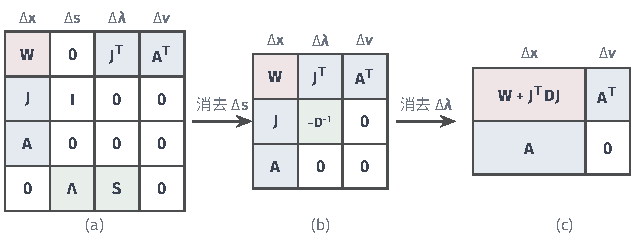
\includegraphics[width=107.5mm]{figures/05-optimization/06-constrained-optimization/tikz/nlipm-kkt-blocks/figure.pdf}
  \caption{Newton方程组的三种等价形式，顶部标出每列对应的方向。红底是含曲率的块，蓝底是约束Jacobian，绿底是对角块，$\bm{D}=\bm{S}^{-1}\bm{\Lambda}$。(a)式~\eqref{eq:nlipm-newton}；(b)消去$\Delta\bm{s}$后的对称鞍点形式；(c)再消去$\Delta\bm{\lambda}$后的压缩形式。}
  \label{fig:nlipm-kkt-blocks}
\end{BookInlineFigure}

把式~\eqref{eq:nlipm-ds}代入式~\eqref{eq:nlipm-dlambda}，再代入第一行，$\Delta\bm{\lambda}$被消去，只剩$\Delta\bm{x}$和$\Delta\bm{\nu}$。记对角矩阵$\bm{D}=\bm{S}^{-1}\bm{\Lambda}$，以及
\begin{equation}
 \tilde{\bm{H}}=\bm{W}+\bm{J}^\top\bm{D}\bm{J},\qquad
 \bm{b}=-\bm{r}_{\mathrm{d}}-\bm{J}^\top\bm{S}^{-1}\bigl(\bm{r}_{\mathrm{c}}+\bm{\Lambda}\bm{r}_{\mathrm{p}}\bigr).
 \label{eq:nlipm-condensed-data}
\end{equation}
方向$\Delta\bm{x}$、$\Delta\bm{\nu}$满足压缩后的鞍点方程
\begin{equation}
 \begin{bmatrix}\tilde{\bm{H}}&\bm{A}^\top\\\bm{A}&\bm{0}\end{bmatrix}
 \begin{bmatrix}\Delta\bm{x}\\\Delta\bm{\nu}\end{bmatrix}
 =\begin{bmatrix}\bm{b}\\-\bm{r}_{\mathrm{e}}\end{bmatrix}.
 \label{eq:nlipm-condensed}
\end{equation}

$\tilde{\bm{H}}$的两部分对应障碍的两种作用：$\bm{J}^\top\bm{D}\bm{J}$在约束法向上加刚度，$\bm{W}$保留目标和约束的弯曲。在式~\eqref{eq:nlipm-newton}的第二种写法里，只消去$\Delta\bm{s}$，保留$\Delta\bm{\lambda}$，得到的矩阵是
\begin{equation}
 \begin{bmatrix}\bm{W}&\bm{J}^\top&\bm{A}^\top\\\bm{J}&-\bm{D}^{-1}&\bm{0}\\\bm{A}&\bm{0}&\bm{0}\end{bmatrix}.
 \label{eq:nlipm-saddle}
\end{equation}
压缩形式维数小，鞍点形式稀疏性好，第~\ref{sec:nlipm-guarantees}节比较它们的代价。

举一个带等式约束的算例，看$\bm{A}$的作用。取下面的矩阵$\tilde{\bm{H}}$和右端$\bm{b}$（稍后的计算过程会在贯穿例的第一轮得到它们），再加一条等式约束$x_1-x_2+1=0$，当前点$(1,2)$满足它，所以$r_{\mathrm{e}}=0$：
\[
 \tilde{\bm{H}}=\begin{bmatrix}7&-2\\-2&9/4\end{bmatrix},\qquad\bm{b}=\begin{bmatrix}8/5\\-19/10\end{bmatrix},\qquad\bm{A}=[1\ \ -1].
\]
由$\bm{A}\Delta\bm{x}=0$，方向只能取$\Delta\bm{x}=\tau(1,1)^\top$。用$(1,1)$左乘第一块方程，$\Delta\nu$相互抵消，得到
\[
 \tfrac{21}{4}\tau=-\tfrac{3}{10},\qquad\text{即}\qquad\tau=-\frac{2}{35}.
\]
再由第一行，$5\tau+\Delta\nu=8/5$，于是$\Delta\nu=66/35$。等式约束的作用是把方向压进切平面，这和第~\ref{chap:quadratic-conic-programming}章的等式约束二次规划一样。

\paragraph{与障碍法的Newton方向比较}
若$\bm{s}=-\bm{g}(\bm{x})$，$\bm{\lambda}=\mu\bm{S}^{-1}\bm{1}$，则$\tilde{\bm{H}}=\nabla^2B_\mu$，两种方法在这一点上的矩阵相同。差别出现在其他点：参数一降，障碍法的乘子估计立刻变成$\mu^+/s_i$，原始—对偶方法的$\lambda_i$则留在当前值，由方程去修正。

回到一维例子，站在$x=-1/2$、$s=3/4$、$\lambda=1$，目标参数$\hat{\mu}=0.05$。这时
\[
 W=2,\quad J=-1,\quad D=\frac43,\quad\tilde{H}=\frac{10}{3},\quad r_{\mathrm{c}}=0.05-0.75=-0.7.
\]
由式~\eqref{eq:nlipm-condensed-data}，$b=-J\,r_{\mathrm{c}}/s=-14/15$，于是
\[
 \Delta x=-0.28,\qquad\Delta s=-0.28,\qquad\Delta\lambda=-0.56.
\]
单位步得到$x=-0.78$、$s=0.47$、$\lambda=0.44$，都留在正确的一侧。同样的起点和目标参数，障碍法的Newton步是$-4.2$。这里的差别和第~\ref{chap:lp-interior-point}章线性化$x_is_i=\mu$而不线性化$s_i=\mu/x_i$是同一个原因。

\paragraph{曲率让残差不再按比例下降}
线性规划中，走步长$\alpha$后等式残差精确地乘以$1-\alpha$。这个性质来自约束是线性的。现在对松弛方程作Taylor展开，走完步长$\alpha$，残差变成
\begin{equation}
 \bm{r}_{\mathrm{p}}^+=(1-\alpha)\bm{r}_{\mathrm{p}}+\bm{\rho}(\alpha),
 \label{eq:nlipm-rp-update}
\end{equation}
其中二阶余项是
\[
 \bm{\rho}(\alpha)=\bm{g}(\bm{x}+\alpha\Delta\bm{x})-\bm{g}(\bm{x})-\alpha\bm{J}\Delta\bm{x}.
\]
若$\nabla g_i$是$L_g$-Lipschitz的，则余项的大小满足
\[
 \lvert\rho_i(\alpha)\rvert\leq\tfrac12L_g\alpha^2\lVert\Delta\bm{x}\rVert_2^2.
\]

贯穿例的$g_1=x_1^2-x_2$是二次的，余项可以精确写出：
\[
 \rho_1(\alpha)=\alpha^2\Delta x_1^2.
\]
图~\ref{fig:nlipm-curved-residual}取一个可行域外的点。线性模型认为约束边界是黄色的切线，走完单位步正好到达；实际约束是抛物线，单位步之后的残差不是零，而是$\Delta x_1^2\approx0.746$。

这个现象还有一个后果：即使当前点满足$\bm{r}_{\mathrm{p}}=\bm{0}$，走一步后也可能变成非零。原始可行性在线性规划中可以一旦达到就永远保持，这里不能。

\begin{BookInlineFigure}
  \centering
  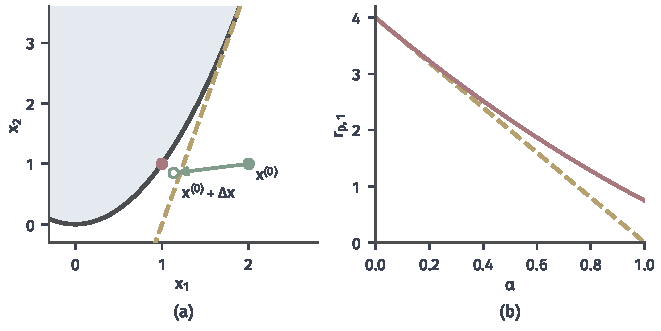
\includegraphics[width=112mm]{figures/05-optimization/06-constrained-optimization/matplotlib/nlipm-curved-residual/figure.pdf}
  \caption{弯的约束使线性化产生误差，贯穿例，起点$\bm{x}^{(0)}=(2,1)$、$\bm{s}=(1,3)$、$\bm{\lambda}=(1,1/3)$、$\sigma=0.2$。(a)深灰粗线是真实边界，黄色虚线是在$\bm{x}^{(0)}$处线性化的边界，绿色箭头是Newton步，红点是$\bm{x}^\star$。(b)红线是实际残差$r_{\mathrm{p},1}$，黄色虚线是线性模型预测的$(1-\alpha)r_{\mathrm{p},1}$，$\alpha=1$时两者相差$\Delta x_1^2$。}
  \label{fig:nlipm-curved-residual}
\end{BookInlineFigure}

\paragraph{线性系统可解，不等于方向好用}
方程组~\eqref{eq:nlipm-condensed}何时有唯一解，答案和约化Hessian有关。

\begin{lemma}[Newton方程的解]
\label{lem:nlipm-newton-solvable}
设$\bm{s},\bm{\lambda}>\bm{0}$，$\bm{A}$满行秩，$\tilde{\bm{H}}$在$\bm{A}$的零空间上正定，即$\bm{A}\bm{d}=\bm{0}$、$\bm{d}\neq\bm{0}$时$\bm{d}^\top\tilde{\bm{H}}\bm{d}>0$。则方程组~\eqref{eq:nlipm-newton}有唯一解。
\end{lemma}

\begin{proof}
消元的每一步都是等价变形，所以只需证明压缩矩阵非奇异。设
\[
 \tilde{\bm{H}}\bm{d}+\bm{A}^\top\bm{w}=\bm{0},\qquad\bm{A}\bm{d}=\bm{0}.
\]
用$\bm{d}^\top$左乘第一式，并用第二式，得到
\[
 \bm{d}^\top\tilde{\bm{H}}\bm{d}=0.
\]
由正定性$\bm{d}=\bm{0}$。于是$\bm{A}^\top\bm{w}=\bm{0}$，由满行秩$\bm{w}=\bm{0}$。
\end{proof}

这个条件比“系数矩阵非奇异”强。矩阵非奇异时方程也有唯一解，但方向可能完全不对。下面的引理说明正定性的真正用途：它保证方向使障碍目标下降。这里的障碍目标把松弛也当作变量，写成
\[
 \psi_{\hat{\mu}}(\bm{x},\bm{s})=f(\bm{x})-\hat{\mu}\sum_{i=1}^m\log s_i.
\]

\begin{lemma}[方向与障碍目标]
\label{lem:nlipm-descent}
设$\bm{r}_{\mathrm{p}}=\bm{0}$，$\bm{r}_{\mathrm{e}}=\bm{0}$，方向由式~\eqref{eq:nlipm-newton}给出，其中目标参数取$\hat{\mu}$。则$\psi_{\hat{\mu}}$沿方向的一阶变化满足
\begin{equation}
 \nabla f^\top\Delta\bm{x}-\hat{\mu}\,\bm{1}^\top\bm{S}^{-1}\Delta\bm{s}=-\Delta\bm{x}^\top\tilde{\bm{H}}\Delta\bm{x}.
 \label{eq:nlipm-descent}
\end{equation}
\end{lemma}

\begin{proof}
由$\bm{r}_{\mathrm{d}}$的定义和$\bm{A}\Delta\bm{x}=\bm{0}$、$\bm{J}\Delta\bm{x}=-\Delta\bm{s}$，有
\[
 \nabla f^\top\Delta\bm{x}=\bm{r}_{\mathrm{d}}^\top\Delta\bm{x}+\bm{\lambda}^\top\Delta\bm{s}.
\]
互补残差满足
\[
 \bm{S}^{-1}\bm{r}_{\mathrm{c}}=\hat{\mu}\bm{S}^{-1}\bm{1}-\bm{\lambda}.
\]
用$\Delta\bm{x}^\top$左乘式~\eqref{eq:nlipm-condensed}的第一块，并代入上式，得到
\[
 \Delta\bm{x}^\top\tilde{\bm{H}}\Delta\bm{x}=-\bm{r}_{\mathrm{d}}^\top\Delta\bm{x}+(\hat{\mu}\bm{S}^{-1}\bm{1}-\bm{\lambda})^\top\Delta\bm{s}.
\]
由第二式解出$\bm{r}_{\mathrm{d}}^\top\Delta\bm{x}$，代入第一式，$\bm{\lambda}^\top\Delta\bm{s}$相互抵消，即得结论。
\end{proof}

所以$\tilde{\bm{H}}$在切空间上不正定时，$\Delta\bm{x}$可能是上升方向。图~\ref{fig:nlipm-regularization}取圆盘外部的例子，$\mu=0.1$，在$\bm{x}=(0.35,1.08)^\top$处的特征值是
\[
 -0.320,\qquad 7.352.
\]
Newton方向的一阶变化是$\nabla B_\mu^\top\bm{d}=+0.947$，它是上升方向，指向鞍点。系数矩阵非奇异，线性方程解得毫无困难，得到的却是错误的方向。

补救办法是\term{矩阵正则化}（matrix regularization）：把$\tilde{\bm{H}}$换成$\tilde{\bm{H}}+\delta_{\mathrm{w}}\bm{I}$，$\delta_{\mathrm{w}}\geq0$逐步增大，直到切空间上正定。例中取$\delta_{\mathrm{w}}=0.47$，新方向的一阶变化是$-2.73$，变成下降方向。

怎样判断切空间上正定？实际中不直接算切空间，而看鞍点矩阵的惯性，即正、负、零特征值的个数。$\bm{A}$满行秩时，$\tilde{\bm{H}}$在零空间上正定，当且仅当矩阵~\eqref{eq:nlipm-condensed}的惯性是$(n,p,0)$。分解$\bm{L}\bm{D}\bm{L}^\top$时可以直接读出惯性，所以试探$\delta_{\mathrm{w}}$只要重复分解。这个判据的证明要用到Sylvester惯性定律，读者可查阅专著\scite{math-nocedal2006numerical}。

\begin{BookInlineFigure}
  \centering
  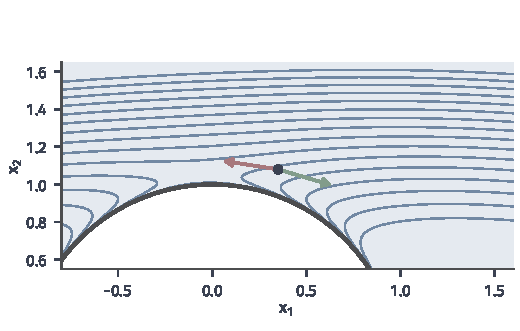
\includegraphics[width=88mm]{figures/05-optimization/06-constrained-optimization/matplotlib/nlipm-regularization/figure.pdf}
  \caption{曲率不定时的方向，圆盘外部的例子，$\mu=0.1$。深灰粗线是约束边界，蓝线是$B_\mu$的等值线，黑点是当前点。红色箭头是未修正的Newton方向，指向上升一侧的鞍点（为便于观察，按比例缩短）；绿色箭头是加上$\delta_{\mathrm{w}}\bm{I}$之后的方向，沿下降方向走向右侧的极小点。}
  \label{fig:nlipm-regularization}
\end{BookInlineFigure}

另一类困难来自约束退化。若活动约束或等式约束的梯度线性相关，$\bm{A}$不再满行秩，矩阵奇异或接近奇异。常用的办法是在右下角加上$-\delta_{\mathrm{c}}\bm{I}$，相当于允许等式约束有微小的违反。数值尺度也要处理：把某条约束乘以$1000$，$\bm{D}$和残差的数值都跟着变，通常先对目标和约束的梯度作缩放。这些修改的代价是方向不再是真正的Newton方向，第~\ref{sec:nlipm-stopping}小节会说明为什么最后要按未经修改的问题检查结果。

\subsection{步长与中心性}
\label{sec:nlipm-step}

得到方向后，还要回答走多远。这里有三件事彼此独立：不能越过边界，这一步要确实有进展，迭代点不能离路径太远。

\paragraph{到边界的比例规则}
第一件事沿用第~\ref{chap:lp-interior-point}章的做法，只是作用在$(\bm{s},\bm{\lambda})$上：
\begin{equation}
 \alpha_{\max}=\min\Bigl\{\min_{\Delta s_i<0}\frac{s_i}{-\Delta s_i},\ \min_{\Delta\lambda_i<0}\frac{\lambda_i}{-\Delta\lambda_i}\Bigr\},\qquad
 \alpha=\min\{1,\ \eta\,\alpha_{\max}\},
 \label{eq:nlipm-alpha}
\end{equation}
其中$\eta\in(0,1)$，没有负分量时约定$\alpha_{\max}=+\infty$。

这条规则保护的是$\bm{s}>\bm{0}$，而不是$\bm{g}(\bm{x})<\bm{0}$。当$\bm{r}_{\mathrm{p}}\neq\bm{0}$时，$\bm{x}$可以暂时越过约束边界。这是原始—对偶方法相对于障碍法的自由，也是第~\ref{sec:nlipm-stopping}小节必须检查原约束的原因。

实现中常对原始变量和对偶变量用不同的步长，因为线性规划中“单一步长让互补量精确下降”的理由在这里已经不成立。下面的算例为了便于手算，仍用单一步长。

\paragraph{残差检验}
满足比例规则的步长仍可能太长，因为式~\eqref{eq:nlipm-rp-update}的余项和$\bm{W}$的变化都没有进入线性模型。最直接的检验是看方程残差有没有变小。把方程组写成$\bm{F}_{\hat{\mu}}(\bm{z})=\bm{0}$，其中$\bm{z}=(\bm{x},\bm{s},\bm{\lambda},\bm{\nu})$，要求
\begin{equation}
 \lVert\bm{F}_{\hat{\mu}}(\bm{z}+\alpha\Delta\bm{z})\rVert_2\leq(1-c\,\alpha)\lVert\bm{F}_{\hat{\mu}}(\bm{z})\rVert_2,
 \label{eq:nlipm-residual-armijo}
\end{equation}
其中$c\in(0,1)$是小常数，不满足时把$\alpha$减半。

\begin{lemma}[Newton方向使残差下降]
\label{lem:nlipm-residual-descent}
设$\bm{F}_{\hat{\mu}}$连续可微，其Jacobian矩阵在$\bm{z}$处非奇异，$\Delta\bm{z}$是Newton方向，$\bm{F}_{\hat{\mu}}(\bm{z})\neq\bm{0}$。则$\alpha>0$足够小时，式~\eqref{eq:nlipm-residual-armijo}成立。
\end{lemma}

\begin{proof}
记
\[
 \Theta(\alpha)=\tfrac12\lVert\bm{F}_{\hat{\mu}}(\bm{z}+\alpha\Delta\bm{z})\rVert_2^2.
\]
由Newton方程$\bm{G}\Delta\bm{z}=-\bm{F}$，其中$\bm{G}$是Jacobian矩阵，有
\[
 \Theta'(0)=\bm{F}^\top\bm{G}\Delta\bm{z}=-\lVert\bm{F}\rVert_2^2.
\]
于是残差范数的展开是
\[
 \sqrt{2\Theta(\alpha)}=\lVert\bm{F}\rVert_2(1-\alpha)+o(\alpha).
\]
而$c<1$，所以$\alpha$足够小时不等式成立。
\end{proof}

这个检验简单，但有明显的盲区：它只看方程残差，分不清极小点和鞍点。方程组的任何解都能把它压到零，包括前面的$x=2$（若不靠正性挡住）和各种局部极大点。所以在非凸问题上，更常用的检验还要看目标。

\paragraph{过滤器}
一个直接想法是把约束违反量和障碍目标合成一个数，用它来比较。这需要一个权重，取大了算法只管可行，取小了只管目标。\term{过滤器}（filter）绕开这个权重，它把每一步看成二维平面上的一个点：
\begin{equation}
 \theta(\bm{z})=\bigl\lVert(\bm{h}(\bm{x}),\ \bm{g}(\bm{x})+\bm{s})\bigr\rVert_2,\qquad
 \psi_\mu(\bm{x},\bm{s})=f(\bm{x})-\mu\sum_{i=1}^m\log s_i.
 \label{eq:nlipm-filter-pair}
\end{equation}

算法保存一些历史点$(\theta_l,\psi_l)$，试探点只要不被其中任何一个点支配，就可以接受，也就是对每个$l$，要么$\theta$比$\theta_l$小，要么$\psi_\mu$比$\psi_l$小。图~\ref{fig:nlipm-filter}中有三个历史点$(0.2,4)$、$(0.5,3)$、$(1,2.5)$。

试探点A$=(0.3,3.2)$的$\theta$比$(0.5,3)$和$(1,2.5)$都小，$\psi_\mu$又比$(0.2,4)$小，所以被接受。试探点B$=(0.6,3.5)$的两个分量都比$(0.5,3)$差，被拒绝。两项指标各有高低的点互不否定，两项都差的点才被淘汰。

实际的过滤器要求有一定幅度的改进，例如$\theta\leq(1-\gamma_\theta)\theta_l$或$\psi_\mu\leq\psi_l-\gamma_\psi\theta_l$，否则可能无穷地接受改进极小的点。如果步长被缩到极小仍不能接受，算法转入\term{可行性恢复}（feasibility restoration）阶段，暂时放下目标，只减小$\theta$。

\begin{BookInlineFigure}
  \centering
  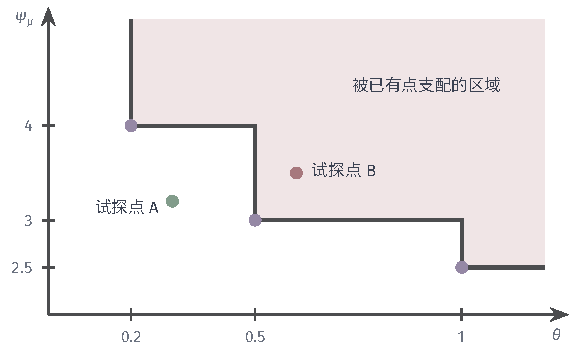
\includegraphics[width=97mm]{figures/05-optimization/06-constrained-optimization/tikz/nlipm-filter/figure.pdf}
  \caption{过滤器。横轴是约束违反量$\theta$，纵轴是障碍目标$\psi_\mu$。紫点是已保存的历史点，红底是被它们支配的区域。绿点A不被任何历史点支配，可以接受；红点B落在被支配区域内，被拒绝。}
  \label{fig:nlipm-filter}
\end{BookInlineFigure}

\paragraph{保持正性与靠近中心是两回事}
到边界的比例规则只保证$s_i,\lambda_i>0$。点可以严格在内部，却让某个乘积比平均值小几千倍，这时下一轮的Newton步很可能被这个小乘积卡住。沿用第~\ref{chap:lp-interior-point}章的度量，定义中心性
\begin{equation}
 \xi=\frac{\min_is_i\lambda_i}{\mu}\in(0,1].
 \label{eq:nlipm-centrality}
\end{equation}
要求$\xi\geq\gamma$（例如$\gamma=10^{-3}$）的集合称为\term{宽邻域}（wide neighborhood）。

图~\ref{fig:nlipm-wspace}把贯穿例的迭代画在$(s_1\lambda_1,s_2\lambda_2)$平面上。中心路径在这个平面上是对角线。绿线取$\sigma=0.2$，$\eta=0.9$，轨迹贴着对角线，中心性最低为$0.49$。

黄线取$\sigma=0.02$，$\eta=0.9999$，每步都几乎走到边界，第一步就让中心性掉到$10^{-3}$，再走两轮才恢复到$0.9$以上。正性两条线都保持了，靠近中心的程度却差别很大。

\begin{BookInlineFigure}
  \centering
  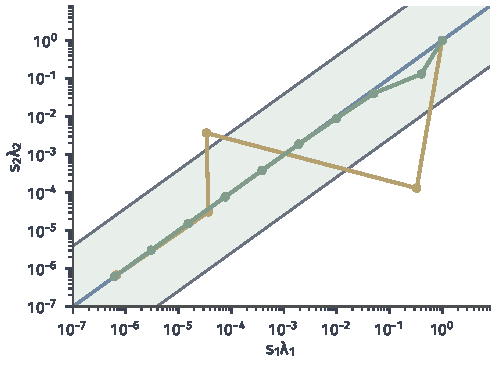
\includegraphics[width=84mm]{figures/05-optimization/06-constrained-optimization/matplotlib/nlipm-wspace/figure.pdf}
  \caption{互补乘积平面，对数坐标，贯穿例。蓝线是$s_1\lambda_1=s_2\lambda_2$，即中心路径；浅绿带是宽邻域$\xi\geq0.05$，灰线是其边界。绿线是$\sigma=0.2$、$\eta=0.9$的迭代，黄线是$\sigma=0.02$、$\eta=0.9999$的迭代，后者离开了浅绿带。}
  \label{fig:nlipm-wspace}
\end{BookInlineFigure}

\paragraph{计算过程}
下面把一轮迭代写成具体步骤，并在例~\eqref{eq:nlipm-running}上逐轮计算。取固定的中心化参数$\sigma=0.2$、比例$\eta=0.9$、残差检验常数$c=10^{-4}$，容差$\varepsilon=10^{-6}$。例中没有等式约束，含$\bm{A}$、$\bm{\nu}$的量都不出现。

\needspace{6\baselineskip}
\paragraph{变量}
\begin{itemize}
 \item $\bm{x}\in\mathbb{R}^n$：原始变量。$\bm{s}\in\mathbb{R}^m$：松弛，全部分量为正。
 \item $\bm{\lambda}\in\mathbb{R}^m$：不等式乘子，全部分量为正。$\bm{\nu}\in\mathbb{R}^p$：等式乘子。
 \item $\mu$、$\hat{\mu}$：平均互补量和本轮的目标参数，由式~\eqref{eq:nlipm-mu}给出。
 \item $\bm{r}_{\mathrm{d}},\bm{r}_{\mathrm{e}},\bm{r}_{\mathrm{p}},\bm{r}_{\mathrm{c}}$：式~\eqref{eq:nlipm-residuals}的四个残差，维数依次是$n$、$p$、$m$、$m$。
 \item $\bm{W}$、$\bm{D}$、$\tilde{\bm{H}}$、$\bm{b}$：Lagrange Hessian、对角缩放、压缩矩阵和右端，分别由式~\eqref{eq:nlipm-lagrange-hessian}、\eqref{eq:nlipm-condensed-data}给出。
 \item $\Delta\bm{x},\Delta\bm{s},\Delta\bm{\lambda},\Delta\bm{\nu}$：本轮的方向；$\alpha_{\max},\alpha$：最大步长和实际步长。
\end{itemize}

\paragraph{初始化}
取$\bm{x}^{(0)}$、$\bm{s}^{(0)}>\bm{0}$、$\bm{\lambda}^{(0)}>\bm{0}$和$\bm{\nu}^{(0)}$，令$t=0$；起点的选取由下一节讨论。例中取严格可行的点，并让两个乘积相等：
\[
 \bm{x}^{(0)}=\begin{bmatrix}1\\2\end{bmatrix},\qquad
 \bm{s}^{(0)}=-\bm{g}(\bm{x}^{(0)})=\begin{bmatrix}1\\2\end{bmatrix},\qquad
 \bm{\lambda}^{(0)}=\begin{bmatrix}1\\1/2\end{bmatrix}.
\]

\needspace{6\baselineskip}
\paragraph{每轮更新}
在第$t$轮，以$(\bm{x}^{(t)},\bm{s}^{(t)},\bm{\lambda}^{(t)},\bm{\nu}^{(t)})$为当前点：
\begin{enumerate}
 \item \textbf{计算残差并检查停止。}按式~\eqref{eq:nlipm-mu}、\eqref{eq:nlipm-residuals}计算$\mu$和残差。若$\lVert\bm{r}_{\mathrm{d}}\rVert_\infty$、$\lVert\bm{r}_{\mathrm{e}}\rVert_\infty$、$\lVert\bm{r}_{\mathrm{p}}\rVert_\infty$和$\max_is_i\lambda_i$都不超过$\varepsilon$，停止并输出当前点。

 例中第一轮$\mu^{(0)}=1$，$\hat{\mu}=0.2$，
 \[
  \bm{r}_{\mathrm{d}}=\begin{bmatrix}-2\\2\end{bmatrix}+\begin{bmatrix}2\\-1/2\end{bmatrix}=\begin{bmatrix}0\\3/2\end{bmatrix},\quad
  \bm{r}_{\mathrm{p}}=\bm{0},\quad
  \bm{r}_{\mathrm{c}}=\begin{bmatrix}-4/5\\-4/5\end{bmatrix}.
 \]

 \item \textbf{形成压缩方程。}由式~\eqref{eq:nlipm-lagrange-hessian}计算$\bm{W}$，由式~\eqref{eq:nlipm-condensed-data}计算$\tilde{\bm{H}}$和$\bm{b}$。检查惯性，必要时加$\delta_{\mathrm{w}}\bm{I}$。

 例中第一轮$\lambda_1=1$，所以$\bm{W}=\operatorname{diag}(3,1)$，而$\bm{D}=\operatorname{diag}(1,1/4)$，$\bm{J}$的两行是$(2,-1)$和$(0,1)$，所以
 \[
  \tilde{\bm{H}}=\begin{bmatrix}3&0\\0&1\end{bmatrix}+\begin{bmatrix}4&-2\\-2&5/4\end{bmatrix}=\begin{bmatrix}7&-2\\-2&9/4\end{bmatrix}.
 \]
 又$\bm{S}^{-1}\bm{r}_{\mathrm{c}}=(-4/5,-2/5)^\top$，于是
 \[
  \bm{b}=-\begin{bmatrix}0\\3/2\end{bmatrix}-\begin{bmatrix}-8/5\\2/5\end{bmatrix}=\begin{bmatrix}8/5\\-19/10\end{bmatrix}.
 \]
 这个矩阵的两个顺序主子式$7$和$47/4$都是正的，因此正定，不需要修正。

 \item \textbf{求方向。}解式~\eqref{eq:nlipm-condensed}得到$\Delta\bm{x}$、$\Delta\bm{\nu}$，再由式~\eqref{eq:nlipm-ds}、\eqref{eq:nlipm-dlambda}回代。

 例中第一轮
 \[
  \Delta\bm{x}=\Bigl(-\frac{4}{235},\,-\frac{202}{235}\Bigr)^\top\approx(-0.0170,\,-0.8596)^\top.
 \]
 回代得到
 \[
  \Delta\bm{s}\approx(-0.8255,\,0.8596)^\top,\qquad\Delta\bm{\lambda}\approx(0.0255,\,-0.6149)^\top.
 \]

 \item \textbf{确定步长。}由式~\eqref{eq:nlipm-alpha}得到候选$\alpha$，再用式~\eqref{eq:nlipm-residual-armijo}（或过滤器）检验，不通过则把$\alpha$减半。

 例中第一轮只有$s_1$和$\lambda_2$在减小，比值分别是$1.2113$和$0.8131$，所以
 \[
  \alpha_{\max}\approx0.8131,\qquad\alpha=0.9\,\alpha_{\max}\approx0.7318.
 \]
 残差范数从$1.8788$降到$0.4559$，检验通过，不需要回溯。

 \item \textbf{更新。}令
 \begin{equation}
  \begin{aligned}
  \bm{x}^{(t+1)}&=\bm{x}^{(t)}+\alpha\Delta\bm{x},\quad&
  \bm{s}^{(t+1)}&=\bm{s}^{(t)}+\alpha\Delta\bm{s},\\
  \bm{\lambda}^{(t+1)}&=\bm{\lambda}^{(t)}+\alpha\Delta\bm{\lambda},\quad&
  \bm{\nu}^{(t+1)}&=\bm{\nu}^{(t)}+\alpha\Delta\bm{\nu},
  \end{aligned}
  \label{eq:nlipm-update}
 \end{equation}
 然后令$t\leftarrow t+1$，回到第1步。

 例中第一轮
 \[
  \begin{gathered}
  \bm{x}^{(1)}\approx(0.9875,\,1.3709)^\top,\\
  \bm{s}^{(1)}\approx(0.3958,\,2.6291)^\top,\qquad\bm{\lambda}^{(1)}\approx(1.0187,\,0.0500)^\top.
  \end{gathered}
 \]
 这时$\bm{r}_{\mathrm{p}}$不再为零，第一个分量是$\alpha^2\Delta x_1^2\approx1.55\times10^{-4}$，这正是式~\eqref{eq:nlipm-rp-update}的余项。
\end{enumerate}

例中第二轮的中间量如下。当前$\mu^{(1)}=0.2673$，$\hat{\mu}=0.0535$，两个乘积是$0.4032$和$0.1314$，于是
\[
 \bm{r}_{\mathrm{d}}\approx(-0.0005,\,0.4022)^\top,\qquad\bm{r}_{\mathrm{c}}\approx(-0.3498,\,-0.0780)^\top.
\]
压缩矩阵和右端是
\[
 \tilde{\bm{H}}\approx\begin{bmatrix}13.076&-5.083\\-5.083&3.592\end{bmatrix},\qquad\bm{b}\approx\begin{bmatrix}1.745\\-1.256\end{bmatrix}.
\]
解方程组并回代，得到
\[
 \begin{gathered}
 \Delta\bm{x}\approx(-0.0054,\,-0.3572)^\top,\\
 \Delta\bm{s}\approx(-0.3467,\,0.3572)^\top,\qquad\Delta\bm{\lambda}\approx(0.0086,\,-0.0365)^\top.
 \end{gathered}
\]
这一轮$\alpha_{\max}\approx1.1418$，$0.9\alpha_{\max}>1$，所以取$\alpha=1$。新的点是
\[
 \begin{gathered}
 \bm{x}^{(2)}\approx(0.9821,\,1.0137)^\top,\\
 \bm{s}^{(2)}\approx(0.0492,\,2.9863)^\top,\qquad\bm{\lambda}^{(2)}\approx(1.0273,\,0.0135)^\top.
 \end{gathered}
\]

此后每轮都取$\alpha=1$，平均互补量几乎每轮乘以$0.2$。表~\ref{tab:nlipm-run}列出全部迭代。第$9$轮后所有残差和乘积都不超过$10^{-6}$，算法停止。

\begin{BookInlineTable}
  \centering
  \footnotesize
  \begin{tabular}{@{}ccccccccc@{}}
    \toprule
    $t$ & $x_1^{(t)}$ & $x_2^{(t)}$ & $s_1^{(t)}$ & $\lambda_1^{(t)}$ & $\mu^{(t)}$ & $\lVert\bm{r}_{\mathrm{d}}\rVert_\infty$ & $\lVert\bm{r}_{\mathrm{p}}\rVert_\infty$ & $\alpha$\\
    \midrule
    0 & 1.0000 & 2.0000 & 1.0000 & 1.0000 & 1.00 & 1.5 & 0 & 0.732\\
    1 & 0.9875 & 1.3709 & 0.3958 & 1.0187 & 0.267 & 0.40 & $1.6\mathrm{e}{-4}$ & 1\\
    2 & 0.9821 & 1.0137 & 0.0492 & 1.0272 & 0.0455 & $9.3\mathrm{e}{-5}$ & $2.9\mathrm{e}{-5}$ & 1\\
    3 & 0.9963 & 1.0023 & 0.0099 & 1.0053 & $9.5\mathrm{e}{-3}$ & $6.2\mathrm{e}{-4}$ & $2.0\mathrm{e}{-4}$ & 1\\
    4 & 0.9993 & 1.0005 & 0.0019 & 1.0011 & $1.9\mathrm{e}{-3}$ & $2.5\mathrm{e}{-5}$ & $8.9\mathrm{e}{-6}$ & 1\\
    5 & 0.9999 & 1.0001 & 0.0004 & 1.0002 & $3.8\mathrm{e}{-4}$ & $1.0\mathrm{e}{-6}$ & $3.4\mathrm{e}{-7}$ & 1\\
    6 & 1.0000 & 1.0000 & 0.0001 & 1.0000 & $7.6\mathrm{e}{-5}$ & $4.1\mathrm{e}{-8}$ & $1.4\mathrm{e}{-8}$ & 1\\
    7 & 1.0000 & 1.0000 & 0.0000 & 1.0000 & $1.5\mathrm{e}{-5}$ & $1.6\mathrm{e}{-9}$ & $5.4\mathrm{e}{-10}$ & 1\\
    8 & 1.0000 & 1.0000 & 0.0000 & 1.0000 & $3.1\mathrm{e}{-6}$ & $6.5\mathrm{e}{-11}$ & $2.2\mathrm{e}{-11}$ & 1\\
    9 & 1.0000 & 1.0000 & 0.0000 & 1.0000 & $6.1\mathrm{e}{-7}$ & $2.6\mathrm{e}{-12}$ & $8.7\mathrm{e}{-13}$ & \\
    \bottomrule
  \end{tabular}
  \caption{贯穿例的逐轮中间量，$\sigma=0.2$、$\eta=0.9$。第$t$行的$\alpha$是从第$t$个点出发那一轮的步长。全部$\alpha$都未经回溯。}
  \label{tab:nlipm-run}
\end{BookInlineTable}

最终得到
\[
 \hat{\bm{x}}\approx(1.0000,\,1.0000)^\top,\qquad\hat{\bm{\lambda}}\approx(1.0000,\,2\times10^{-7})^\top,
\]
目标误差约$6.1\times10^{-7}$。第$3$轮的驻定残差比第$2$轮大，这说明残差并不单调下降，因为每轮的目标$\hat{\mu}$都在变。

图~\ref{fig:nlipm-iterates}比较这条轨迹与障碍法（$\tau=0.2$）。两者起点相同，绿线直接朝解走，$9$轮停止；黄线先走到$\mu=1$的碗底，再沿路径前进，在同样的精度下用了$34$个Newton步。图~\ref{fig:nlipm-residual-curves}给出各残差随轮次的变化，可以看到$\lVert\bm{r}_{\mathrm{p}}\rVert_\infty$从零升起，这是约束弯曲带来的。

\begin{BookInlineFigure}
  \centering
  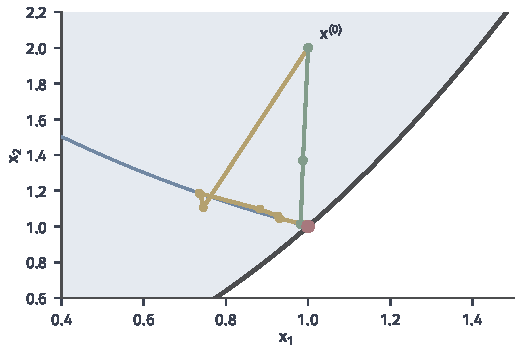
\includegraphics[width=88mm]{figures/05-optimization/06-constrained-optimization/matplotlib/nlipm-iterates/figure.pdf}
  \caption{贯穿例的迭代点，局部放大。蓝线是中心路径，绿线是$\sigma=0.2$的原始—对偶迭代，黄线是$\tau=0.2$的障碍法的Newton迭代点，红点是$\bm{x}^\star$，深灰粗线是约束边界。两者都从$(1,2)$出发。}
  \label{fig:nlipm-iterates}
\end{BookInlineFigure}

\begin{BookInlineFigure}
  \centering
  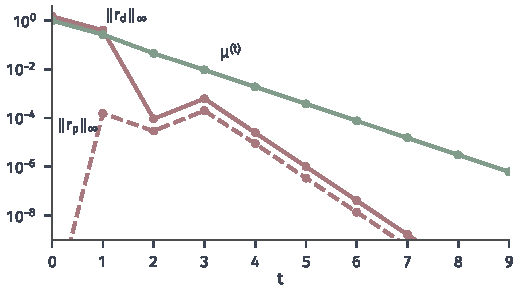
\includegraphics[width=88mm]{figures/05-optimization/06-constrained-optimization/matplotlib/nlipm-residual-curves/figure.pdf}
  \caption{贯穿例的残差历史，对数纵轴。红色实线是$\lVert\bm{r}_{\mathrm{d}}\rVert_\infty$，红色虚线是$\lVert\bm{r}_{\mathrm{p}}\rVert_\infty$（第$0$轮为零，图中从下方进入），绿线是$\mu^{(t)}$。}
  \label{fig:nlipm-residual-curves}
\end{BookInlineFigure}

\paragraph{预测—校正要重新核对条件}
第~\ref{chap:lp-interior-point}章的预测—校正可以直接搬用：先解$\sigma=0$的方程组，用试走后的互补量选$\sigma$，再把$\Delta s_i^{\mathrm{a}}\Delta\lambda_i^{\mathrm{a}}$移到右端。两次求解共用一次分解。例中第一轮，预测步的结果是
\[
 \alpha^{\mathrm{a}}\approx0.7015,\qquad\mu^{\mathrm{a}}\approx0.1640,\qquad\sigma\approx0.0044.
\]
校正后取到$\alpha\approx0.8556$，平均互补量降到$0.2085$，而固定$\sigma=0.2$时是$0.2673$。代价也很明显：两个乘积变成$0.0997$和$0.3174$，不再相等。

搬用时有三点要重新核对。校正项只补偿了互补方程的二阶项，约束的二阶余项$\bm{\rho}$并没有补偿。预测步用的$\bm{W}$若经过了正则化，二阶项的估计就是另一个问题的量。线性规划中单位步之后等式残差恰好消失，这里没有这个性质，所以校正之后的步长仍要过残差或过滤器的检验，单靠比例规则不够。

\section{初始化与精度}
\label{sec:nlipm-init-accuracy}

前两节都假设手里已经有一个能用的起点，也没有说算到什么程度可以停。本节要回答这两个问题：障碍路径和原始—对偶迭代分别需要怎样的起点，以及停下来的点能对原问题说什么。

\subsection{初始点的构造}
\label{sec:nlipm-initial-point}

两类方法对起点的要求不同。障碍法要计算$\log(-g_i(\bm{x}))$，所以每个迭代点都必须严格可行。原始—对偶方法的方程里不出现$\log(-g_i)$，它只要求$\bm{s},\bm{\lambda}>\bm{0}$，$\bm{x}$可以在可行域之外。

\paragraph{辅助可行性问题}
需要严格可行点时，可以先解一个以“最大违反量”为目标的问题：
\begin{equation}
 \min_{\bm{x},\rho}\ \rho\quad\text{s.t.}\quad g_i(\bm{x})\leq\rho\ (i=1,\ldots,m),\quad\bm{h}(\bm{x})=\bm{0}.
 \label{eq:nlipm-phase-one}
\end{equation}
这个问题的严格可行点是现成的：只要有一个满足等式的$\bm{x}$，取$\rho>\max_ig_i(\bm{x})$即可。线性等式可以解线性方程组得到这样的$\bm{x}$，非线性等式本身就是一个方程求根的问题，这里并没有绕过它。

设$\rho^\star$是最优值。在凸问题上，它的符号给出三种结论：

\begin{itemize}
 \item $\rho^\star<0$：最优点严格可行，可以作为障碍法的起点。
 \item $\rho^\star=0$：原问题可行或处在可行的边缘，但没有严格可行点。
 \item $\rho^\star>0$：原问题不可行。
\end{itemize}

在非凸问题上，算法只能找到局部解，$\rho>0$的局部解不能说明原问题不可行。

贯穿例从$\bm{x}^{(0)}=(2,1)^\top$开始，$\bm{g}=(3,-3)^\top$，取$\rho=4$就严格可行。解$\min\max\{x_1^2-x_2,\ x_2-4\}$时，$x_1=0$使第一项最小，再让$-x_2=x_2-4$，得到
\[
 \bm{x}=(0,2)^\top,\qquad\rho^\star=-2.
\]
这正是解析中心。图~\ref{fig:nlipm-phase-one}显示，随着$\rho$减小，放宽后的区域逐层收缩到这一点。实际上不必解到最优，一旦$\rho<0$就可以提前停下，这时得到的点已经是严格可行的。

\begin{BookInlineFigure}
  \centering
  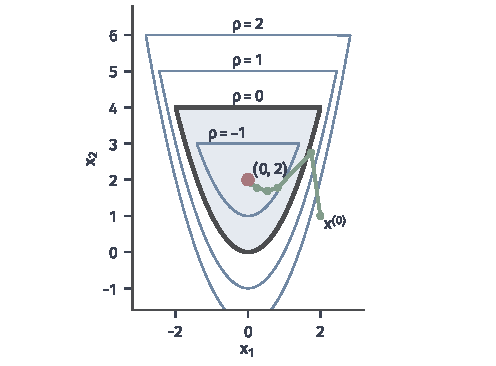
\includegraphics[width=84mm]{figures/05-optimization/06-constrained-optimization/matplotlib/nlipm-phase-one/figure.pdf}
  \caption{贯穿例的辅助问题~\eqref{eq:nlipm-phase-one}。蓝线是$\max_ig_i(\bm{x})=\rho$的水平集，深灰粗线是$\rho=0$，即原可行集的边界。绿线是从可行域外的$\bm{x}^{(0)}=(2,1)$出发、用障碍法解这个问题的迭代点，红点是解$(0,2)$，这里$\rho^\star=-2$。}
  \label{fig:nlipm-phase-one}
\end{BookInlineFigure}

\paragraph{从非零的原始残差开始}
原始—对偶方法不用先解辅助问题。任取$\bm{x}^{(0)}$，再选一个正的下限$\delta$，令
\begin{equation}
 s_i^{(0)}=\max\bigl\{-g_i(\bm{x}^{(0)}),\ \delta\bigr\},\qquad\lambda_i^{(0)}=\frac{\mu^{(0)}}{s_i^{(0)}}.
 \label{eq:nlipm-infeasible-start}
\end{equation}
这样所有乘积都等于$\mu^{(0)}$，起点在互补方程的意义下是居中的。约束已满足的分量，$\bm{r}_{\mathrm{p}}$是零，被违反的分量，$\bm{r}_{\mathrm{p}}$非零。

要记住的是，$\bm{s},\bm{\lambda}>\bm{0}$并不意味着$\bm{g}(\bm{x})+\bm{s}=\bm{0}$已经成立。正性是起点就满足的，松弛方程是迭代要逐步解的。在$\bm{r}_{\mathrm{p}}\neq\bm{0}$的点上，$s_i>0$也不告诉我们$g_i(\bm{x})<0$。

贯穿例取$\bm{x}^{(0)}=(2,1)^\top$，$\delta=1$，$\mu^{(0)}=1$，由式~\eqref{eq:nlipm-infeasible-start}得到
\[
 \bm{s}^{(0)}=\begin{bmatrix}1\\3\end{bmatrix},\qquad\bm{\lambda}^{(0)}=\begin{bmatrix}1\\1/3\end{bmatrix},\qquad\bm{r}_{\mathrm{p}}=\begin{bmatrix}4\\0\end{bmatrix}.
\]
仍取$\sigma=0.2$，按式~\eqref{eq:nlipm-condensed-data}算出
\[
 \tilde{\bm{H}}=\begin{bmatrix}19&-4\\-4&19/9\end{bmatrix},\qquad\bm{b}\approx\begin{bmatrix}-15.8\\3.133\end{bmatrix}.
\]
解出方向并回代，得到
\[
 \Delta\bm{x}\approx(-0.8636,\,-0.1521)^\top,\qquad\Delta\bm{s}\approx(-0.6977,\,0.1521)^\top.
\]

这一轮取到$\alpha=1$。线性规划中单位步会让等式残差归零，这里第一个分量却变成$\Delta x_1^2\approx0.7458$，这就是图~\ref{fig:nlipm-curved-residual}(b)的右端点。

第二轮$\alpha\approx0.946$，$r_{\mathrm{p},1}$降到$0.059$，再一轮之后降到$1.7\times10^{-5}$。图~\ref{fig:nlipm-infeasible-start}显示，残差下降虽然不再是精确的比例，但在这个例子上很快就跟上了互补量。

\begin{BookInlineFigure}
  \centering
  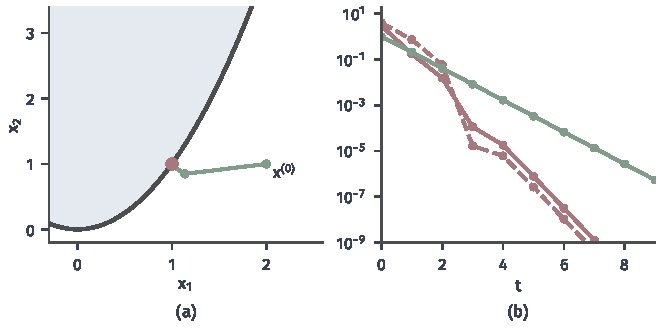
\includegraphics[width=112mm]{figures/05-optimization/06-constrained-optimization/matplotlib/nlipm-infeasible-start/figure.pdf}
  \caption{从可行域外启动，贯穿例，$\sigma=0.2$、$\eta=0.9$。(a)绿线是迭代点，从$(2,1)$进入可行域附近，红点是$\bm{x}^\star$。(b)红色虚线是$\lVert\bm{r}_{\mathrm{p}}\rVert_\infty$，红色实线是$\lVert\bm{r}_{\mathrm{d}}\rVert_\infty$，绿线是$\mu^{(t)}$。}
  \label{fig:nlipm-infeasible-start}
\end{BookInlineFigure}

\paragraph{不收敛到可行点的情形}
线性化的约束可能和当前的残差彼此矛盾。看不可行的一维约束$g(x)=x^2+1\leq0$。残差$x^2+1+s$在$s>0$上没有零点，迭代会被吸引到$x=0$、$s\to0$，这一点上$J=2x=0$，线性化的约束不再能改变残差。这是约束违反量的一个驻点，不是原问题的解。

对凸问题，这样的点可以变成证书。若存在$\bm{w}\geq\bm{0}$，使$\inf_{\bm{x}}\sum_iw_ig_i(\bm{x})>0$，则约束一定无解，因为可行点会让这个和不大于零。上面的例子取$w=1$，$\inf_x(x^2+1)=1>0$。非凸问题没有这样的结论，算法停在不可行驻点时，只能报告“这一带没有找到可行点”。

\paragraph{缺少严格可行点或约束退化}
内点法依赖的几个条件可能在模型层面就不成立，这时调参数没有用，要回到模型。图~\ref{fig:nlipm-no-interior}是三种常见情形。

图(a)的约束是两个相切的圆盘：
\[
 x_1^2+(x_2-1)^2\leq1,\qquad x_1^2+(x_2+1)^2\leq1.
\]
可行集只有原点，$\bm{C}^{\circ}$是空集。若目标是$\min x_1$，原点是唯一的可行点，但$\nabla f=(1,0)^\top$无法写成$(0,-2)^\top$和$(0,2)^\top$的组合，KKT条件不成立。这时根本没有路径。

图(b)是把一条等式拆成两条不等式，内部同样是空的。这种情形只需把等式约束显式写出来。

图(c)是重复的约束，例如把$g_1\leq0$写了两遍。这时$\bm{C}^{\circ}$不空，沿路径两个乘子相等，极限却不满足线性无关：在极限点，乘子的方向$(1,-1)$落在Newton矩阵的零空间里，矩阵奇异。算法的表现是$\bm{D}$很大的时候矩阵越来越病态，需要预处理去掉重复约束，或者加上$\delta_{\mathrm{c}}$。

\begin{BookInlineFigure}
  \centering
  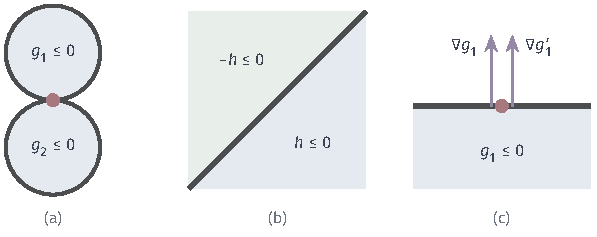
\includegraphics[width=101mm]{figures/05-optimization/06-constrained-optimization/tikz/nlipm-no-interior/figure.pdf}
  \caption{内点法的条件在模型层面失效的三种情形。(a)两个相切的圆盘（浅蓝），可行集只有红点，没有内部。(b)$h\leq0$和$-h\leq0$的公共部分是深灰的直线，同样没有内部。(c)同一条约束写了两遍，紫色箭头是两个相同的梯度，它们线性相关，乘子不唯一。}
  \label{fig:nlipm-no-interior}
\end{BookInlineFigure}

\subsection{停止条件}
\label{sec:nlipm-stopping}

迭代点永远在内部，算法只能在某处停下。这一小节回答什么量决定停止，以及停下的点能保证什么。

\paragraph{三项分别评价}
对参数$\mu$，定义误差
\begin{equation}
 E_\mu(\bm{z})=\max\Bigl\{\frac{\lVert\bm{r}_{\mathrm{d}}\rVert_\infty}{c_{\mathrm{d}}},\ \lVert\bm{r}_{\mathrm{e}}\rVert_\infty,\ \lVert\bm{r}_{\mathrm{p}}\rVert_\infty,\ \frac{\lVert\bm{S}\bm{\Lambda}\bm{1}-\mu\bm{1}\rVert_\infty}{c_{\mathrm{c}}}\Bigr\},
 \label{eq:nlipm-error}
\end{equation}
这里$c_{\mathrm{d}},c_{\mathrm{c}}\geq1$是按乘子大小确定的缩放，防止乘子很大时要求过严，贯穿例中都取$1$。$E_\mu$度量子问题的误差，$E_0$才度量原问题的KKT误差。最后的判据是$E_0\leq\varepsilon$。

\paragraph{参数小不等于解好了}
一个很小的$\mu$什么都说明不了，因为$\mu$是算法自己设定的数。起点取$\bm{\lambda}=10^{-3}\bm{1}$，$\mu$立刻就很小，而$\bm{r}_{\mathrm{d}}$的大小是$2$。反过来，$E_\mu$很小也只说明子问题解得好。

图~\ref{fig:nlipm-stop-staircase}是贯穿例上的一次运行，每当$E_\mu\leq0.1\mu$时，令$\mu\leftarrow0.2\mu$。第$6$轮$E_\mu\approx1.3\times10^{-5}$，子问题已经解得很准，而$E_0=0.04$，正好是当时的$\mu$。可以看到$E_0$紧贴$\mu$下降，$E_\mu$每次更新参数后跳起，再快速下降。

\begin{BookInlineFigure}
  \centering
  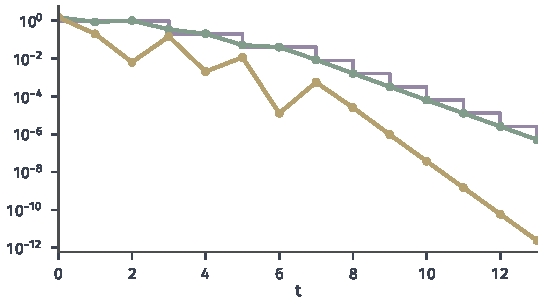
\includegraphics[width=92mm]{figures/05-optimization/06-constrained-optimization/matplotlib/nlipm-stop-staircase/figure.pdf}
  \caption{子问题误差与原问题误差，贯穿例，$\mu$只在$E_\mu\leq0.1\mu$时按$0.2$倍减小，对数纵轴。紫色折线是当前的$\mu$，绿线是原问题的KKT误差$E_0$，黄线是子问题误差$E_\mu$。$E_\mu$很小的时候，$E_0$仍然停在$\mu$的水平上。}
  \label{fig:nlipm-stop-staircase}
\end{BookInlineFigure}

\paragraph{内层精度与外层参数的配合}
由定义，$\lvert E_0-E_\mu\rvert\leq\mu/c_{\mathrm{c}}$，所以把$E_\mu$解得比$\mu$小很多并没有好处，$E_0$反正停在$\mu$的量级。常用的规则是：内层解到$E_\mu\leq\kappa\mu$，再更新参数
\begin{equation}
 \mu^+=\max\Bigl\{\frac{\varepsilon}{10},\ \min\bigl\{\tau\mu,\ \mu^{1+\theta}\bigr\}\Bigr\},
 \label{eq:nlipm-mu-update}
\end{equation}
其中$\kappa>0$，$\tau\in(0,1)$，$\theta\in(0,1)$。$\mu$大时线性减小，$\mu$小时超线性减小。下限$\varepsilon/10$防止参数比容差小太多，否则$\bm{D}$的数值徒然变大，矩阵更病态，而精度并不提高。

\paragraph{近似点能保证什么}
下面的定理说明残差小怎样转化成目标误差，它把定理~\ref{thm:nlipm-gap}推广到迭代点不在路径上、残差不为零的情形。

\begin{theorem}[近似点的目标误差]
\label{thm:nlipm-approx-certificate}
设$f$、$g_i$凸且可微，$\bm{h}(\bm{x})=\bm{A}\bm{x}-\bm{b}$，$(\bm{x},\bm{s},\bm{\lambda},\bm{\nu})$满足$\bm{\lambda}\geq\bm{0}$，残差如式~\eqref{eq:nlipm-residuals}定义。设$\bm{x}^\star$是最优解，$R\geq\lVert\bm{x}-\bm{x}^\star\rVert_2$。则
\begin{equation}
 f(\bm{x})-f^\star\leq\bm{\lambda}^\top\bm{s}-\bm{\lambda}^\top\bm{r}_{\mathrm{p}}-\bm{\nu}^\top\bm{r}_{\mathrm{e}}+\lVert\bm{r}_{\mathrm{d}}\rVert_2R.
 \label{eq:nlipm-approx-upper}
\end{equation}
若$(\bm{\lambda}^\star,\bm{\nu}^\star)$是一组KKT乘子，则还有
\begin{equation}
 f(\bm{x})-f^\star\geq-(\bm{\lambda}^\star)^\top\bm{g}(\bm{x})-(\bm{\nu}^\star)^\top\bm{r}_{\mathrm{e}}.
 \label{eq:nlipm-approx-lower}
\end{equation}
\end{theorem}

\begin{proof}
由$\bm{\lambda}\geq\bm{0}$和$\bm{x}^\star$可行，有
\[
 f^\star\geq\mathcal{L}(\bm{x}^\star,\bm{\lambda},\bm{\nu}).
\]
函数$\mathcal{L}(\cdot,\bm{\lambda},\bm{\nu})$是凸的，在$\bm{x}$处的梯度是$\bm{r}_{\mathrm{d}}$，于是
\[
 \mathcal{L}(\bm{x}^\star,\bm{\lambda},\bm{\nu})\geq\mathcal{L}(\bm{x},\bm{\lambda},\bm{\nu})+\bm{r}_{\mathrm{d}}^\top(\bm{x}^\star-\bm{x})\geq\mathcal{L}(\bm{x},\bm{\lambda},\bm{\nu})-\lVert\bm{r}_{\mathrm{d}}\rVert_2R.
\]
代入$\bm{g}(\bm{x})=\bm{r}_{\mathrm{p}}-\bm{s}$和$\bm{h}(\bm{x})=\bm{r}_{\mathrm{e}}$，$\mathcal{L}(\bm{x},\bm{\lambda},\bm{\nu})$展开为
\[
 f(\bm{x})-\bm{\lambda}^\top\bm{s}+\bm{\lambda}^\top\bm{r}_{\mathrm{p}}+\bm{\nu}^\top\bm{r}_{\mathrm{e}}.
\]
整理即得式~\eqref{eq:nlipm-approx-upper}。

对下界，$\bm{x}^\star$是凸函数$\mathcal{L}(\cdot,\bm{\lambda}^\star,\bm{\nu}^\star)$的最小点，并且由互补，这个最小值等于$f^\star$，于是
\[
 f^\star\leq\mathcal{L}(\bm{x},\bm{\lambda}^\star,\bm{\nu}^\star)=f(\bm{x})+(\bm{\lambda}^\star)^\top\bm{g}(\bm{x})+(\bm{\nu}^\star)^\top\bm{h}(\bm{x}).
\]
移项即得式~\eqref{eq:nlipm-approx-lower}。
\end{proof}

式~\eqref{eq:nlipm-approx-upper}右端的第一项是互补量，其余三项是残差被乘子和距离放大的部分。这正是第~\ref{chap:lp-interior-point}章不可行点上间隙公式的非线性版本。下界说明，点略微不可行时目标可以低于$f^\star$，低的幅度由违反量乘以最优乘子决定。

用表~\ref{tab:nlipm-run}中$t=4$的点核对。这时互补量和两个残差项是
\[
 \bm{\lambda}^\top\bm{s}\approx3.82\times10^{-3},\quad\lvert\bm{\lambda}^\top\bm{r}_{\mathrm{p}}\rvert\approx8.9\times10^{-6},\quad\lVert\bm{r}_{\mathrm{d}}\rVert_2\approx2.5\times10^{-5}.
\]
可行集的直径不超过$4.5$，取$R=4.5$，上界约为$3.92\times10^{-3}$。实际误差是$1.92\times10^{-3}$，确实在界内。

\paragraph{始终按原问题报告}
内点法的内部变量经过松弛、缩放，矩阵可能经过正则化，交付时都要回到原问题上算一遍。可行性按$\max_i\max\{g_i(\bm{x}),0\}$和$\lVert\bm{h}(\bm{x})\rVert_\infty$计算，而不是$\lVert\bm{r}_{\mathrm{p}}\rVert_\infty$，因为$s_i>0$时残差小并不排除$g_i(\bm{x})$略大于零。互补按$\lambda_i\lvert g_i(\bm{x})\rvert$计算，驻定按未缩放的梯度计算。

三种常见的修改都可能制造假象。矩阵正则化只改变方向，不改变残差的定义，所以它本身不影响判据，但$\delta_{\mathrm{c}}$较大时迭代可能停在一个并不满足等式的点上。把约束放宽成$g_i\leq\epsilon$的实现，要说明放宽量。恢复步骤之后乘子往往被重置，这时要用新的乘子重新计算$\bm{r}_{\mathrm{d}}$，不能沿用恢复之前的数值。

收敛到一个$E_0$很小的点，在非凸问题上也只说明这一点近似满足KKT条件。若需要二阶信息，还要看最后一次分解时是否用过$\delta_{\mathrm{w}}>0$，用过说明约化Hessian在该点并不正定。

\section{锥规划中的障碍}
\label{sec:nlipm-conic}

有些约束写成标量不等式并不自然。$\lVert\bm{u}\rVert_2\leq t$在$\bm{u}=\bm{0}$处不可微，矩阵正定更是一个无法用有限条光滑不等式简单表达的条件。接下来要弄清：怎样为这些集合直接造一个障碍，路径跟踪的哪些操作可以照搬，哪些不能？

\paragraph{共同的框架}
第~\ref{chap:quadratic-conic-programming}章的锥规划写成
\begin{equation}
 \min_{\bm{x}}\ \langle\bm{c},\bm{x}\rangle\quad\text{s.t.}\quad\mathcal{A}\bm{x}=\bm{b},\quad\bm{x}\in\bm{K},
 \label{eq:nlipm-conic-primal}
\end{equation}
其中$\bm{K}$是闭凸锥，$\mathcal{A}$是线性映射。它的对偶问题是
\begin{equation}
 \max_{\bm{y},\bm{z}}\ \bm{b}^\top\bm{y}\quad\text{s.t.}\quad\mathcal{A}^*\bm{y}+\bm{z}=\bm{c},\quad\bm{z}\in\bm{K}^*,
 \label{eq:nlipm-conic-dual}
\end{equation}
$\bm{K}^*$是对偶锥，$\mathcal{A}^*$是$\mathcal{A}$的伴随映射，$\bm{z}$的角色就是第~\ref{chap:lp-interior-point}章的对偶松弛。可行点上目标差仍是$\langle\bm{x},\bm{z}\rangle$。

设$\phi$是定义在$\bm{K}$内部的障碍函数。障碍问题$\min\langle\bm{c},\bm{x}\rangle+\mu\phi(\bm{x})$的一阶条件给出$\bm{c}+\mu\nabla\phi(\bm{x})=\mathcal{A}^*\bm{y}$。令$\bm{z}=\bm{c}-\mathcal{A}^*\bm{y}$，得到中心路径的方程
\begin{equation}
 \mathcal{A}\bm{x}=\bm{b},\qquad\mathcal{A}^*\bm{y}+\bm{z}=\bm{c},\qquad\bm{z}=-\mu\nabla\phi(\bm{x}).
 \label{eq:nlipm-conic-central}
\end{equation}
第三式就是互补方程的一般形式。取$\phi=-\sum_i\log x_i$，它就是$x_iz_i=\mu$。

间隙由障碍的一个性质决定。设$\phi$满足$\phi(\tau\bm{x})=\phi(\bm{x})-\vartheta\log\tau$，对所有$\tau>0$成立。对$\tau$求导再令$\tau=1$，得到
\[
 \langle\nabla\phi(\bm{x}),\bm{x}\rangle=-\vartheta.
\]
代入式~\eqref{eq:nlipm-conic-central}，沿路径的间隙是
\begin{equation}
 \langle\bm{x},\bm{z}\rangle=\vartheta\mu.
 \label{eq:nlipm-conic-gap}
\end{equation}
数$\vartheta$称为\term{障碍参数}（barrier parameter），它取代了线性规划中的$n$和本章前面的$m$。

\subsection{二阶锥障碍}
\label{sec:nlipm-soc}

记$\bm{x}=(\bm{u},t)$，$\bm{u}\in\mathbb{R}^{q}$，$t\in\mathbb{R}$，第~\ref{chap:quadratic-conic-programming}章的二阶锥是$\{(\bm{u},t):\lVert\bm{u}\rVert_2\leq t\}$。它的内部由$t>\lVert\bm{u}\rVert_2$给出，等价于$t>0$且$t^2-\lVert\bm{u}\rVert_2^2>0$。

\begin{definition}[二阶锥障碍]
\label{def:nlipm-soc-barrier}
记$\bm{R}=\operatorname{diag}(-\bm{I}_q,1)$，$\omega(\bm{x})=\bm{x}^\top\bm{R}\bm{x}$。在二阶锥内部定义
\begin{equation}
 \phi(\bm{x})=-\log\omega(\bm{x})=-\log\bigl(t^2-\lVert\bm{u}\rVert_2^2\bigr).
 \label{eq:nlipm-soc-barrier}
\end{equation}
\end{definition}

点靠近锥面时$\omega\downarrow0$，$\phi\to+\infty$，一整张锥面只用一项对数表达。由$\omega(\tau\bm{x})=\tau^2\omega(\bm{x})$，这个障碍的参数是$\vartheta=2$，与维数$q$无关。

\paragraph{导数}
由$\nabla\omega=2\bm{R}\bm{x}$、$\nabla^2\omega=2\bm{R}$和复合函数法则，得到
\begin{equation}
 \nabla\phi(\bm{x})=-\frac{2\bm{R}\bm{x}}{\omega},\qquad
 \nabla^2\phi(\bm{x})=\frac{4\bm{R}\bm{x}\bm{x}^\top\bm{R}}{\omega^2}-\frac{2\bm{R}}{\omega}.
 \label{eq:nlipm-soc-derivatives}
\end{equation}
$\bm{R}$不定，所以第二项不定，正定性要靠两项配合。

\begin{lemma}[二阶锥障碍的Hessian正定]
\label{lem:nlipm-soc-pd}
在二阶锥内部，$\nabla^2\phi(\bm{x})\succ\bm{0}$。
\end{lemma}

\begin{proof}
取非零的$\bm{d}=(\bm{v},r)$。考察二次函数
\[
 p(\beta)=(\bm{d}+\beta\bm{x})^\top\bm{R}(\bm{d}+\beta\bm{x})=\omega\beta^2+2\beta\,\bm{x}^\top\bm{R}\bm{d}+\bm{d}^\top\bm{R}\bm{d}.
\]
取$\beta_0=-r/t$，向量$\bm{d}+\beta_0\bm{x}$的最后一个分量为零，所以
\[
 p(\beta_0)=-\lVert\bm{v}+\beta_0\bm{u}\rVert_2^2\leq0.
\]
又$\omega>0$，所以$p$有实根，判别式非负，这就是
\[
 (\bm{x}^\top\bm{R}\bm{d})^2\geq\omega\,\bm{d}^\top\bm{R}\bm{d}.
\]

由式~\eqref{eq:nlipm-soc-derivatives}，Hessian的二次型是
\[
 \bm{d}^\top\nabla^2\phi\bm{d}=\frac{4(\bm{x}^\top\bm{R}\bm{d})^2}{\omega^2}-\frac{2\bm{d}^\top\bm{R}\bm{d}}{\omega}.
\]
若$\bm{d}^\top\bm{R}\bm{d}>0$，代入判别式不等式，它不小于$2\bm{d}^\top\bm{R}\bm{d}/\omega>0$。

若$\bm{d}^\top\bm{R}\bm{d}\leq0$，两项都非负。两项同时为零时，$\bm{d}^\top\bm{R}\bm{d}=0$且$\bm{x}^\top\bm{R}\bm{d}=0$，于是
\[
 p(\beta)=\omega\beta^2.
\]
结合$p(\beta_0)\leq0$，得$\beta_0=0$，即$r=0$。这时$p(\beta_0)=0$给出$\bm{v}=\bm{0}$，与$\bm{d}\neq\bm{0}$矛盾。
\end{proof}

用一个二维的点核对，取$q=1$，$\bm{x}=(u,t)=(1,2)$，这时$\omega=3$。由式~\eqref{eq:nlipm-soc-derivatives}，
\[
 \nabla\phi=\begin{bmatrix}2/3\\-4/3\end{bmatrix},\qquad
 \nabla^2\phi=\frac19\begin{bmatrix}10&-8\\-8&10\end{bmatrix}.
\]
Hessian的特征值是$2/9$和$2$，都是正的。

\paragraph{允许的步长}
沿方向$\bm{d}=(\bm{v},r)$走到$\bm{x}+\alpha\bm{d}$，$\omega$是$\alpha$的二次函数：
\begin{equation}
 \omega(\alpha)=\omega+2\alpha\,\bm{x}^\top\bm{R}\bm{d}+\alpha^2\,\bm{d}^\top\bm{R}\bm{d}.
 \label{eq:nlipm-soc-step}
\end{equation}
$\alpha_{\max}$是使$t+\alpha r>0$的前提下$\omega(\alpha)$的最小正根。这和线性规划的比值检验是同一件事，只是一次方程换成了二次方程，仍然有精确的公式，不需要试探。

例中取$\bm{d}=(2,-1)$，式~\eqref{eq:nlipm-soc-step}给出
\[
 \omega(\alpha)=3-8\alpha-3\alpha^2=(1-3\alpha)(3+\alpha).
\]
最小正根是$\alpha_{\max}=1/3$，对应锥面上的点$(5/3,5/3)$。沿这条线，$\phi$的两个导数是$8/3$和$82/9$，图~\ref{fig:nlipm-soc-barrier}(b)的黄线就是这个二次模型，它在边界处仍是有限值，真正的障碍趋于无穷。

\begin{BookInlineFigure}
  \centering
  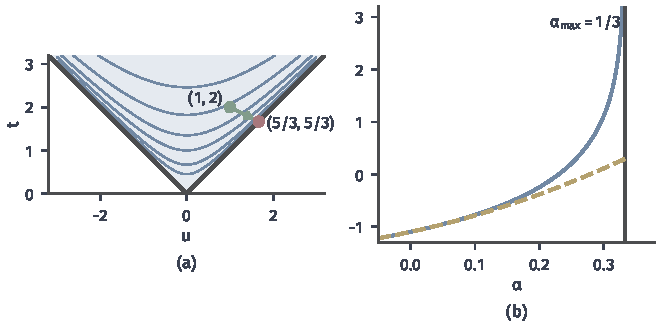
\includegraphics[width=112mm]{figures/05-optimization/06-constrained-optimization/matplotlib/nlipm-soc-barrier/figure.pdf}
  \caption{二阶锥（$q=1$）的障碍。(a)浅蓝区域是锥内部，深灰粗线是锥面，蓝线是$\phi$的等值线。绿点是$(1,2)$，绿色箭头是方向$(2,-1)$，红点是它到达锥面的位置$(5/3,5/3)$。(b)沿该方向的$\phi$（蓝线）与它在$\alpha=0$处的二次模型（黄色虚线），深灰粗线是$\alpha_{\max}=1/3$。}
  \label{fig:nlipm-soc-barrier}
\end{BookInlineFigure}

\paragraph{仿射映射进入锥后的Newton系统}
实际问题的约束通常写成
\[
 \lVert\bm{B}\bm{x}+\bm{e}\rVert_2\leq\bm{a}^\top\bm{x}+d,
\]
也就是$\bm{y}(\bm{x})=\bm{Q}\bm{x}+\bm{q}$落在锥中，这里$\bm{Q}$由$\bm{B}$和$\bm{a}^\top$拼成，$\bm{q}=(\bm{e},d)$。由链式法则，
\begin{equation}
 \nabla_{\bm{x}}\phi=\bm{Q}^\top\nabla\phi(\bm{y}),\qquad
 \nabla_{\bm{x}}^2\phi=\bm{Q}^\top\nabla^2\phi(\bm{y})\bm{Q}.
 \label{eq:nlipm-soc-affine}
\end{equation}

把式~\eqref{eq:nlipm-soc-derivatives}代入，得到的矩阵是“稀疏的$\bm{Q}^\top\bm{R}\bm{Q}$”加上一个秩一矩阵。秩一项的向量$\bm{Q}^\top\bm{R}\bm{y}$通常是稠密的，直接相加会填满矩阵。保留锥结构的实现把它单独存放，或者在鞍点矩阵中增加一行一列，这样既不丢失稀疏性，也能用现成的分解。

\paragraph{展开成标量约束的代价}
也可以把约束写成标量不等式$g(\bm{u},t)=\lVert\bm{u}\rVert_2-t\leq0$，用本章前几节的方法。问题出在$\bm{u}=\bm{0}$：$g$在这里不可微，而这恰恰可能是解所在的位置，例如目标要把$\lVert\bm{B}\bm{x}+\bm{e}\rVert_2$压到零时。图~\ref{fig:nlipm-soc-kink}显示，$-\log(t-\lVert\bm{u}\rVert_2)$在$\bm{u}=\bm{0}$处有折角，$-\log(t^2-\lVert\bm{u}\rVert_2^2)$却是光滑的，因为它用平方把折角消掉了。

改写成$g=\lVert\bm{u}\rVert_2^2-t^2\leq0$并不解决问题。这个$g$不是凸函数，它的零下水平集还包括$t<0$的另一半锥，所以必须同时约束$t\geq0$。二阶锥障碍用$\omega$的同时把定义域限定在$t>0$的内部，避免了这两个麻烦。

\begin{BookInlineFigure}
  \centering
  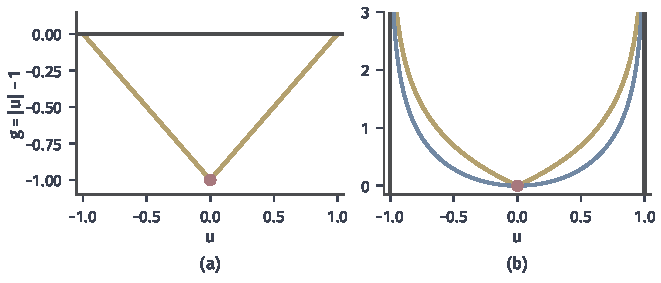
\includegraphics[width=112mm]{figures/05-optimization/06-constrained-optimization/matplotlib/nlipm-soc-kink/figure.pdf}
  \caption{标量写法与锥障碍，$t=1$。(a)标量约束$g=\lvert u\rvert-1$在$u=0$处有折角（红点）。(b)黄线是$-\log(1-\lvert u\rvert)$，保留了折角；蓝线是二阶锥障碍$-\log(1-u^2)$，在$u=0$处光滑。深灰粗线是边界。}
  \label{fig:nlipm-soc-kink}
\end{BookInlineFigure}

\subsection{半正定锥障碍}
\label{sec:nlipm-psd}

变量换成对称矩阵$\bm{X}\in\mathcal{S}^n$，约束是$\bm{X}\succeq\bm{0}$，内积是迹内积
\[
 \langle\bm{X},\bm{Z}\rangle=\operatorname{tr}(\bm{X}\bm{Z}).
\]
半正定锥在这个内积下是自对偶的，所以$\bm{K}^*=\bm{K}$。

\paragraph{特征值逼近零}
$\bm{X}$越靠近边界，最小的特征值越接近零。记$\bm{X}$的特征值为$\rho_1,\ldots,\rho_n>0$，对每个特征值都放一项对数障碍，得到
\begin{equation}
 \phi(\bm{X})=-\sum_{i=1}^n\log\rho_i(\bm{X})=-\log\det\bm{X}.
 \label{eq:nlipm-psd-barrier}
\end{equation}
计算时不必求特征值，$\log\det$可以由Cholesky分解得到。由$\det(\tau\bm{X})=\tau^n\det\bm{X}$，障碍参数是$\vartheta=n$。

\paragraph{线性扰动下的导数}
沿对称方向$\bm{D}$看。因为$\bm{X}\succ\bm{0}$，可以写成
\[
 \bm{X}+\alpha\bm{D}=\bm{X}^{1/2}\bigl(\bm{I}+\alpha\bm{X}^{-1/2}\bm{D}\bm{X}^{-1/2}\bigr)\bm{X}^{1/2}.
\]
记$\bm{X}^{-1/2}\bm{D}\bm{X}^{-1/2}$的特征值为$\beta_1,\ldots,\beta_n$，它们也是$\bm{X}^{-1}\bm{D}$的特征值。取行列式再取对数，得到
\begin{equation}
 \phi(\bm{X}+\alpha\bm{D})=\phi(\bm{X})-\sum_{i=1}^n\log(1+\alpha\beta_i).
 \label{eq:nlipm-psd-expansion}
\end{equation}
对$\alpha$展开到二阶，一阶系数是$-\sum_i\beta_i$，二阶系数是$\sum_i\beta_i^2$。写成迹，就是
\begin{equation}
 \begin{gathered}
 \langle\nabla\phi(\bm{X}),\bm{D}\rangle=-\operatorname{tr}(\bm{X}^{-1}\bm{D}),\\
 \langle\bm{D},\nabla^2\phi(\bm{X})[\bm{D}]\rangle=\operatorname{tr}(\bm{X}^{-1}\bm{D}\bm{X}^{-1}\bm{D}).
 \end{gathered}
 \label{eq:nlipm-psd-derivatives}
\end{equation}
所以在迹内积下$\nabla\phi(\bm{X})=-\bm{X}^{-1}$，Hessian是线性算子$\bm{D}\mapsto\bm{X}^{-1}\bm{D}\bm{X}^{-1}$。

式~\eqref{eq:nlipm-psd-expansion}同时给出最大步长。$\bm{X}+\alpha\bm{D}\succ\bm{0}$当且仅当每个$1+\alpha\beta_i>0$，所以若$\beta_{\min}<0$，
\begin{equation}
 \alpha_{\max}=-\frac{1}{\beta_{\min}},
 \label{eq:nlipm-psd-step}
\end{equation}
否则$\alpha_{\max}=+\infty$。

用具体的矩阵算一遍。取
\[
 \bm{X}=\begin{bmatrix}2&1\\1&2\end{bmatrix},\qquad\bm{D}=\begin{bmatrix}-1&-1\\-1&-2\end{bmatrix}.
\]
$\bm{X}$的特征值是$1$和$3$。直接计算，
\[
 \bm{X}^{-1}\bm{D}=\frac13\begin{bmatrix}-1&0\\-1&-3\end{bmatrix},
\]
它的特征值是$-1/3$和$-1$，所以$\alpha_{\max}=1$。可以核对，$\bm{X}+\bm{D}$的第二行是零，确实落在边界上。

由式~\eqref{eq:nlipm-psd-derivatives}，一阶、二阶导数分别是
\[
 \frac13+1=\frac43,\qquad\frac19+1=\frac{10}{9}.
\]
而$\det(\bm{X}+\alpha\bm{D})=(1-\alpha)(3-\alpha)$，对$-\log$直接求导得到同样的数。图~\ref{fig:nlipm-psd-barrier}显示了特征值沿这个方向的变化和障碍的上升。

\begin{BookInlineFigure}
  \centering
  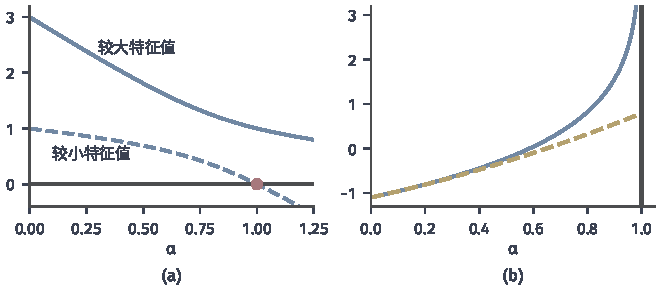
\includegraphics[width=112mm]{figures/05-optimization/06-constrained-optimization/matplotlib/nlipm-psd-barrier/figure.pdf}
  \caption{半正定锥的障碍，沿$\bm{X}+\alpha\bm{D}$。(a)$\bm{X}+\alpha\bm{D}$的两个特征值，红点是较小的特征值到达零的位置$\alpha_{\max}=1$，深灰粗线是零。(b)蓝线是$-\log\det(\bm{X}+\alpha\bm{D})$，黄色虚线是它在$\alpha=0$处的二次模型，深灰粗线是$\alpha_{\max}$。}
  \label{fig:nlipm-psd-barrier}
\end{BookInlineFigure}

\paragraph{矩阵的互补不能照搬标量操作}
中心路径的第三式是$\bm{Z}=\mu\bm{X}^{-1}$，等价于$\bm{X}\bm{Z}=\mu\bm{I}$。标量情形下，线性化$x_is_i=\mu$毫无歧义。矩阵情形下，直接线性化得到
\begin{equation}
 \Delta\bm{X}\,\bm{Z}+\bm{X}\Delta\bm{Z}=\sigma\mu\bm{I}-\bm{X}\bm{Z}.
 \label{eq:nlipm-psd-linearize}
\end{equation}
麻烦在于$\bm{X}$和$\bm{Z}$不交换，$\bm{X}\bm{Z}$一般不对称。解出来的$\Delta\bm{X}$也不对称，走一步之后$\bm{X}$就离开了对称矩阵空间。

看一个具体的例子。取前面的$\bm{X}$，再取$\bm{Z}=\operatorname{diag}(1,2)$，对偶方向$\Delta\bm{Z}$是非对角的对称矩阵。由式~\eqref{eq:nlipm-psd-linearize}解$\Delta\bm{X}$时，出现的项是
\[
 \bm{X}\Delta\bm{Z}\bm{Z}^{-1}=\begin{bmatrix}2&1\\1&2\end{bmatrix}\begin{bmatrix}0&1\\1&0\end{bmatrix}\begin{bmatrix}1&0\\0&1/2\end{bmatrix}=\begin{bmatrix}1&1\\2&1/2\end{bmatrix},
\]
它不是对称的。

解决的办法是\term{原始—对偶缩放}（primal-dual scaling）：选一个可逆矩阵$\bm{P}$，不线性化$\bm{X}\bm{Z}$，而线性化对称化之后的量
\begin{equation}
 \mathcal{H}_{\bm{P}}(\bm{M})=\tfrac12\bigl(\bm{P}\bm{M}\bm{P}^{-1}+(\bm{P}\bm{M}\bm{P}^{-1})^\top\bigr),\qquad
 \mathcal{H}_{\bm{P}}(\bm{X}\bm{Z})=\mu\bm{I}.
 \label{eq:nlipm-psd-scaling}
\end{equation}
三种选择最常见：$\bm{P}=\bm{I}$只把结果对称化；$\bm{P}=\bm{Z}^{1/2}$称为HKM方向；$\bm{P}$取Nesterov—Todd缩放矩阵时，$\bm{X}$与$\bm{Z}$被映到同一个矩阵。不同选择的方向不同，都要保证$\Delta\bm{X}$、$\Delta\bm{Z}$是对称的。

以HKM方向为例，把$\Delta\bm{X}$对称化之后，得到
\[
 \Delta\bm{X}=\sigma\mu\bm{Z}^{-1}-\bm{X}-\tfrac12\bigl(\bm{X}\Delta\bm{Z}\bm{Z}^{-1}+\bm{Z}^{-1}\Delta\bm{Z}\bm{X}\bigr).
\]
代入约束，形成关于$\Delta\bm{y}$的方程，系数矩阵的元素是
\begin{equation}
 M_{ij}=\operatorname{tr}\bigl(\bm{A}_i\bm{X}\bm{A}_j\bm{Z}^{-1}\bigr),
 \label{eq:nlipm-psd-schur}
\end{equation}
其中$\bm{A}_i$是约束$\langle\bm{A}_i,\bm{X}\rangle=b_i$的系数矩阵。它是第~\ref{chap:lp-interior-point}章$\bm{A}\bm{D}\bm{A}^\top$的矩阵版本。

\paragraph{内积配对要保持一致}
实现中常把对称矩阵排成向量，这一步很容易出错。$\bm{X}$有$n(n+1)/2$个独立元素，若直接取上三角排成向量，内积就变了。前面的$\bm{X}$满足$\operatorname{tr}(\bm{X}^2)=10$，而向量$(2,1,2)$的平方和是$9$，因为非对角元在迹里算了两次。

正确的做法是把非对角元乘以$\sqrt{2}$，得到$(2,\sqrt{2},2)$，平方和正好是$10$。对偶变量、梯度和$\mathcal{A}^*$都要用同样的约定，否则对偶可行性和间隙算的都不是原来的量。

\paragraph{三种障碍的对比}
表~\ref{tab:nlipm-barriers}把本章的三种障碍放在一起。形式相同的地方是路径和间隙的公式，不同的地方在互补的写法和步长的求法，这两处决定了线性代数的结构。

\begin{BookInlineTable}
  \centering
  \footnotesize
  \begin{tabular}{@{}llll@{}}
    \toprule
    量 & 标量$s>0$ & 二阶锥 & 半正定锥\\
    \midrule
    障碍 & $-\log s$ & $-\log(t^2-\lVert\bm{u}\rVert_2^2)$ & $-\log\det\bm{X}$\\
    参数$\vartheta$ & $1$ & $2$ & $n$\\
    $-\nabla\phi$ & $1/s$ & $2\bm{R}\bm{x}/\omega$ & $\bm{X}^{-1}$\\
    内积 & 乘法 & 欧氏内积 & 迹内积\\
    $\alpha_{\max}$ & 比值 & 二次方程的根 & $\bm{X}^{-1}\bm{D}$的特征值\\
    线性代数 & 对角 & 对角加秩一 & 稠密缩放矩阵\\
    \bottomrule
  \end{tabular}
  \caption{三种锥的障碍及相应的计算。}
  \label{tab:nlipm-barriers}
\end{BookInlineTable}

\section{保证与计算成本}
\label{sec:nlipm-guarantees}

第~\ref{chap:lp-interior-point}章证明了线性规划上短步路径跟踪的迭代界。这就需要回答：这个结果在什么条件下能够推广，在什么情形下必须退回局部结论，以及每一轮实际要花多少计算？

\paragraph{为什么要有一个比光滑更强的条件}
Newton法的通常分析用Hessian的Lipschitz常数$M$，结论依赖坐标的选取。障碍函数在边界附近的三阶导数趋于无穷，$M$根本不存在一个有限的整体值。路径跟踪的分析需要一种随点变化的尺子。

用$\phi$自己的Hessian当尺子。下面的条件要求三阶导数被二阶导数控制，这就是\term{自协调}（self-concordant）。

\begin{definition}[自协调障碍]
\label{def:nlipm-self-concordant}
设$\phi$是开凸集上三阶连续可微的凸函数，在边界附近趋于$+\infty$。记$\phi'$、$\phi''$、$\phi'''$为沿方向$\bm{d}$的方向导数。若对所有点和所有方向，
\begin{equation}
 \lvert\phi'''\rvert\leq2(\phi'')^{3/2},\qquad(\phi')^2\leq\vartheta\,\phi'',
 \label{eq:nlipm-self-concordant}
\end{equation}
就称$\phi$是参数为$\vartheta$的自协调障碍。
\end{definition}

对$\phi(x)=-\log x$，沿$d=1$的三个导数是$-1/x$、$1/x^2$、$-2/x^3$。代入两个不等式，都恰好取等号，其中$\vartheta=1$。第一个不等式的两边在缩放$x$时变化相同，所以这个条件不依赖坐标的单位。

三种基本的障碍都是自协调的：$m$条线性约束的对数障碍参数是$m$，二阶锥障碍参数是$2$，$n\times n$半正定锥障碍参数是$n$。凸二次约束的$-\log(-g)$也是自协调的，参数是$1$，所以贯穿例的障碍参数是$\vartheta=2$。

\paragraph{Dikin椭球：局部模型信多远}
自协调的直接后果是，以$\nabla^2\phi$定义的单位椭球落在定义域内：
\begin{equation}
 \bigl\{\bm{x}+\bm{d}:\bm{d}^\top\nabla^2\phi(\bm{x})\bm{d}<1\bigr\}\subset\operatorname{dom}\phi.
 \label{eq:nlipm-dikin}
\end{equation}
这个集合称为\term{Dikin椭球}（Dikin ellipsoid）。多面体的情形可以直接验证：$\bm{g}(\bm{x})=\bm{A}\bm{x}-\bm{b}$时，二次型等于$\sum_i(\bm{a}_i^\top\bm{d}/s_i)^2$。它小于$1$，就有每个$\lvert\bm{a}_i^\top\bm{d}\rvert<s_i$，于是新点的每个松弛都还是正的。

一般情形的证明需要沿线段积分第一个不等式，读者可查阅专著\scite{math-boyd2004convex}。

图~\ref{fig:nlipm-dikin}画出贯穿例的四个Dikin椭球，在椭球边界上逐点计算，松弛都是正的。靠近边界时椭球在法向变扁，在切向仍然较长。这就是局部模型“信多远”的答案，随位置自动调整，不需要知道全局的光滑常数。

\begin{BookInlineFigure}
  \centering
  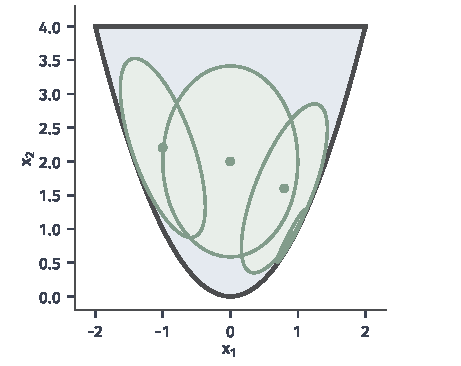
\includegraphics[width=78mm]{figures/05-optimization/06-constrained-optimization/matplotlib/nlipm-dikin/figure.pdf}
  \caption{贯穿例的Dikin椭球，绿点是四个基点，绿色曲线是$\bm{d}^\top\nabla^2\phi(\bm{x})\bm{d}=1$围成的椭球。四个椭球都留在可行集（浅蓝）之内，靠近边界的椭球更扁。}
  \label{fig:nlipm-dikin}
\end{BookInlineFigure}

\paragraph{凸问题的迭代界}
有了这把尺子，第~\ref{chap:lp-interior-point}章的短步分析可以整体推广，其中$\sqrt{n}$换成$\sqrt{\vartheta}$。结论如下，证明要用到自协调函数的Newton减量分析，篇幅较长，读者可查阅专著\scite{math-boyd2004convex}。

\begin{theorem}[路径跟踪的迭代次数]
\label{thm:nlipm-complexity}
设目标是线性函数，可行集有界且有严格可行点，$\phi$是参数为$\vartheta$的自协调障碍，起点足够靠近路径。则短步路径跟踪得到$\varepsilon$精度的解所需的Newton步数为
\begin{equation}
 O\Bigl(\sqrt{\vartheta}\,\log\frac{\vartheta\mu^{(0)}}{\varepsilon}\Bigr).
 \label{eq:nlipm-complexity}
\end{equation}
\end{theorem}

这个界不依赖$f$和$g_i$的条件数，只依赖$\vartheta$，这是内点法在凸问题上最强的结论。目标非线性时，可以用上图形式把它移进约束，代价是要为新的约束找到自协调障碍。

式~\eqref{eq:nlipm-complexity}也解释了为什么锥结构有价值。一个$q+1$维的二阶锥只贡献$\vartheta=2$，如果把它拆成很多线性不等式去逼近，$\vartheta$就随拆分的条数增长。

\paragraph{线性规划的结论不能外推}
多项式界依赖两件事：约束有容易计算的自协调障碍，并且问题是凸的。两者都可能不成立。

第一，凸性并不自动给出自协调。取$g(x)=\mathrm{e}^x-1\leq0$，障碍$\phi=-\log(1-\mathrm{e}^x)$是凸函数，但$x\to-\infty$时$\phi''$和$\phi'''$都约等于$\mathrm{e}^x$，于是
\[
 \frac{\lvert\phi'''\rvert}{(\phi'')^{3/2}}\approx\mathrm{e}^{-x/2}\to\infty.
\]
第一个不等式不可能成立。每个开凸集都存在参数为$O(n)$的自协调障碍，但这是存在性的结果，这样的障碍一般无法计算。

第二，非凸问题求全局解是NP难的，非凸二次规划就已经如此，所以不可能有类似式~\eqref{eq:nlipm-complexity}的全局结果，除非$\mathrm{P}=\mathrm{NP}$。

\paragraph{非凸问题的局部收敛}
非凸问题上能证明的是：在定理~\ref{thm:nlipm-local-path}的条件下，从足够近的点出发，Newton迭代跟着路径收敛到KKT点。下面给出一步的估计。记$\bm{z}^\star$为该KKT点及其松弛、乘子，$\bm{F}_\mu(\bm{z})=\bm{F}_0(\bm{z})-\mu\bm{e}$，其中$\bm{e}$只在互补方程处为$1$，$\bm{G}$是$\bm{F}_0$的Jacobian矩阵。

\begin{theorem}[Newton步的局部估计]
\label{thm:nlipm-local-rate}
设定理~\ref{thm:nlipm-local-path}的条件成立，$\nabla^2f$、$\nabla^2g_i$、$\nabla^2h_j$在$\bm{x}^\star$附近是$M$-Lipschitz的。则存在$\bm{z}^\star$的邻域和常数$C_{\mathrm{G}}$、$M_{\mathrm{G}}$、$C_{\mathrm{p}}$（$M_{\mathrm{G}}$由$M$和乘子的界决定），使邻域内的$\bm{z}$和足够小的$\mu^+>0$满足：单位Newton步
\begin{equation}
 \bm{z}^+=\bm{z}-\bm{G}(\bm{z})^{-1}\bm{F}_{\mu^+}(\bm{z})
 \label{eq:nlipm-local-step}
\end{equation}
有
\begin{equation}
 \lVert\bm{z}^+-\bm{z}^\star\rVert_2\leq\frac{C_{\mathrm{G}}M_{\mathrm{G}}}{2}\bigl(\lVert\bm{z}-\bm{z}^\star\rVert_2+C_{\mathrm{p}}\mu^+\bigr)^2+C_{\mathrm{p}}\mu^+.
 \label{eq:nlipm-local-rate}
\end{equation}
\end{theorem}

\begin{proof}
定理~\ref{thm:nlipm-local-path}的证明说明$\bm{G}(\bm{z}^\star)$非奇异，所以在邻域内
\[
 \lVert\bm{G}(\bm{z})^{-1}\rVert_2\leq C_{\mathrm{G}}.
\]
$\bm{G}$的各块由$\nabla f$、$\nabla^2f$、$\nabla^2g_i$、$\nabla^2h_j$和乘子组成，因此在邻域内是$M_{\mathrm{G}}$-Lipschitz的。路径连续可微，所以
\[
 \lVert\bm{z}(\mu)-\bm{z}^\star\rVert_2\leq C_{\mathrm{p}}\mu.
\]

记$\bm{z}'=\bm{z}(\mu^+)$，它满足$\bm{F}_{\mu^+}(\bm{z}')=\bm{0}$。由Newton步的定义，
\[
 \bm{z}^+-\bm{z}'=\bm{G}(\bm{z})^{-1}\Bigl[\bm{G}(\bm{z})(\bm{z}-\bm{z}')-\bigl(\bm{F}_{\mu^+}(\bm{z})-\bm{F}_{\mu^+}(\bm{z}')\bigr)\Bigr].
\]
方括号内是一阶Taylor余项，由$\bm{G}$的Lipschitz性，它的范数不超过$\tfrac12M_{\mathrm{G}}\lVert\bm{z}-\bm{z}'\rVert_2^2$。于是
\[
 \lVert\bm{z}^+-\bm{z}'\rVert_2\leq\tfrac12C_{\mathrm{G}}M_{\mathrm{G}}\lVert\bm{z}-\bm{z}'\rVert_2^2.
\]
由三角不等式，$\bm{z}$到$\bm{z}'$的距离满足
\[
 \lVert\bm{z}-\bm{z}'\rVert_2\leq\lVert\bm{z}-\bm{z}^\star\rVert_2+C_{\mathrm{p}}\mu^+.
\]
再对$\bm{z}^+$用一次三角不等式，即得结论。
\end{proof}

式~\eqref{eq:nlipm-local-rate}右端有两项：Newton法自身的二次项，以及目标参数的偏移。$\mu^+$与当前误差同阶时，收敛是线性的，表~\ref{tab:nlipm-run}中$\sigma$固定为$0.2$，误差每轮大约乘以$0.2$，就是这种情形。按式~\eqref{eq:nlipm-mu-update}让$\mu^+$超线性减小，收敛速度也变成超线性。

这个估计假设单位步可以走，定理本身没有保证这一点，还要证明$\alpha=1$满足比例规则：活动约束的$s_i$和不活动约束的$\lambda_i$都是$O(\mu)$量级的小量，方向也必须是相应量级，这需要参数更新不能太快，也需要$\eta\to1$。完整的论证较长，读者可查阅专著\scite{math-nocedal2006numerical}。

\paragraph{全局的情形}
从任意点出发，非凸问题上能证明的是：在迭代点有界、矩阵经过惯性修正、约束正则等假设下，带过滤器或合成目标检验的算法的极限点要么满足KKT条件，要么是约束违反量的驻点。这里没有全局最优的保证，图~\ref{fig:nlipm-nonconvex-fold}已经说明，路径本身可能走向较差的局部解。表~\ref{tab:nlipm-claims}总结了两类问题上结论的区别。

\begin{BookInlineTable}
  \centering
  \footnotesize
  \begin{tabular}{@{}lll@{}}
    \toprule
    问题 & 凸问题 & 一般非凸问题\\
    \midrule
    路径 & 整条存在且唯一 & 只在KKT点附近\\
    路径上的间隙 & $f-f^\star\leq m\mu$ & 无全局含义\\
    迭代界 & 自协调时$\sqrt{\vartheta}$型 & 无\\
    停止的含义 & 近似全局解的证书 & 近似KKT点\\
    不可行的判定 & 可给证书 & 只能报告局部驻点\\
    局部速度 & 超线性 & 正则性下超线性\\
    \bottomrule
  \end{tabular}
  \caption{内点法在凸问题与非凸问题上的结论。}
  \label{tab:nlipm-claims}
\end{BookInlineTable}

\paragraph{每一轮的代价}
一轮的工作分三块：计算$f$、$\bm{g}$、$\bm{h}$及其一二阶导数，分解线性系统，以及可能的回溯。回溯只重新计算函数值，比较便宜。决定性的是分解。

压缩矩阵$\tilde{\bm{H}}=\bm{W}+\bm{J}^\top\bm{D}\bm{J}$是$n\times n$的。若有一条约束涉及很多变量，$\bm{J}$有一个稠密的行，$\bm{J}^\top\bm{D}\bm{J}$就是稠密的。鞍点形式~\eqref{eq:nlipm-saddle}维数大，却保留了稀疏性。

图~\ref{fig:nlipm-sparse-fill}是一个$n=m=20$的算例，$\bm{J}$是双对角的，最后一行稠密，共$58$个非零元，取$\bm{W}=\bm{I}$。压缩矩阵完全稠密，它的下三角因子有$210$个非零元。$40\times40$的鞍点矩阵把稠密行排在最后，下三角因子只有$117$个非零元。

这和第~\ref{chap:lp-interior-point}章的$\bm{A}\bm{D}\bm{A}^\top$是同一个现象，只是这里还多了$\bm{W}$。稠密情形下，$n\times n$的分解需要约$n^3/3$次运算；鞍点矩阵不定，要用$\bm{L}\bm{D}\bm{L}^\top$分解和主元选择，主元顺序会随数值改变，符号分析不能像线性规划那样只做一次。每试一个$\delta_{\mathrm{w}}$就要重新分解一次。

\begin{BookInlineFigure}
  \centering
  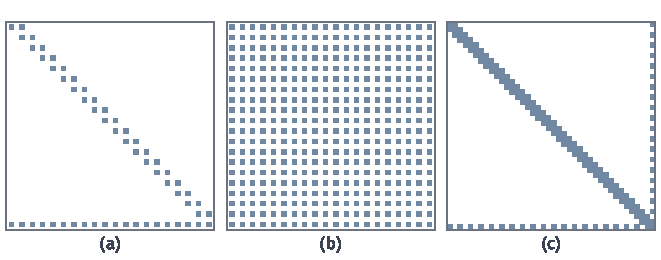
\includegraphics[width=112mm]{figures/05-optimization/06-constrained-optimization/matplotlib/nlipm-sparse-fill/figure.pdf}
  \caption{三个矩阵的非零模式，蓝点表示非零元。(a)$20\times20$的Jacobian矩阵，双对角加上一个稠密行。(b)压缩矩阵$\bm{W}+\bm{J}^\top\bm{D}\bm{J}$，完全稠密。(c)鞍点矩阵$[\bm{W},\bm{J}^\top;\bm{J},-\bm{D}^{-1}]$，变量与约束交错排列，稠密行排在最后。}
  \label{fig:nlipm-sparse-fill}
\end{BookInlineFigure}

\paragraph{条件数}
$\bm{D}$的对角元是$\lambda_i/s_i$。$\mu\to0$时，活动约束上它约为$(\lambda_i^\star)^2/\mu$，趋于无穷，不活动约束上它约为$\mu/(s_i^\star)^2$，趋于零，矩阵的条件数按$1/\mu$增长。

图~\ref{fig:nlipm-cond-growth}显示，贯穿例的压缩矩阵和鞍点矩阵都是如此，保留鞍点结构并不能消除这种病态，它的好处在稀疏性。这种病态的结构很特殊，向后稳定的直接分解能够得到足够准确的方向；迭代法就没有这样幸运，共轭梯度类的方法在$\mu$小时需要专门的预条件子。

\begin{BookInlineFigure}
  \centering
  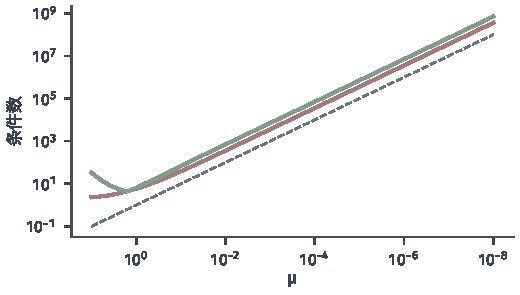
\includegraphics[width=88mm]{figures/05-optimization/06-constrained-optimization/matplotlib/nlipm-cond-growth/figure.pdf}
  \caption{贯穿例沿中心路径的条件数，横轴是$\mu$，向右减小。红线是压缩矩阵$\tilde{\bm{H}}$，绿线是鞍点矩阵，灰色虚线是参照线$1/\mu$。两条曲线都按$1/\mu$增长。}
  \label{fig:nlipm-cond-growth}
\end{BookInlineFigure}

\paragraph{外层轮数}
总代价等于外层轮数乘以每轮的分解代价。实际问题上，原始—对偶方法通常几十轮结束，这是经验而不是定理，它在式~\eqref{eq:nlipm-complexity}的界之下很多。

与第~\ref{chap:feasible-iterations}章的可行迭代和第~\ref{chap:penalty-multiplier-methods}章的乘子方法相比，内点法每轮的代价高，轮数少。能够精确分解时，内点法很有优势；分解太贵、只能得到低精度解就够时，一阶方法更合适。

\section{本章小结}
\label{sec:nlipm-summary}

本章开头的问题是，约束变弯之后，线性规划的路径跟踪还剩下什么。骨架都留下了：在不等式上加对数障碍，驻定条件给出扰动互补$s_i\lambda_i=\mu$，让$\mu$减小到零。等式约束没有内部，仍要显式保留。

新增的内容来自曲率。障碍的Hessian多了$\nabla^2g_i/(-g_i)$一项，Newton系统左上角多了Lagrange Hessian，松弛方程的残差不再按$1-\alpha$的比例下降。非凸时，矩阵可能在切空间上不正定，解方程得到的方向可能是上升方向，要靠惯性检查和矩阵正则化修正，再由残差检验或过滤器决定接受哪一步。

内部性、中心性和最优性是三种不同的检查对象。$\bm{s},\bm{\lambda}>\bm{0}$由到边界的比例规则维护，中心性由$\sigma$和邻域控制，最优性只能由驻定残差、约束残差和互补量共同判断。很小的$\mu$或很小的$E_\mu$都不是原问题的结论，最后要按未经修改的问题报告。

起点有两种。障碍路径需要严格可行点，可以用辅助问题求出；原始—对偶迭代只要求$\bm{s},\bm{\lambda}>\bm{0}$，可以从非零残差出发。没有严格内点、约束重复或线性相关时，问题出在模型上，需要单独检查。

二阶锥和半正定锥有各自的障碍$-\log(t^2-\lVert\bm{u}\rVert_2^2)$和$-\log\det\bm{X}$，路径和间隙的形式不变，$n$换成障碍参数$\vartheta$。步长由二次方程或特征值给出。矩阵互补不能照搬标量操作，$\Delta\bm{X}$要经缩放保持对称，内积配对也要前后一致。

能给出什么结论，由模型的条件决定。凸问题上有整条路径、间隙$m\mu$、近似点的误差界，自协调时还有$\sqrt{\vartheta}$型的迭代界。一般非凸问题只有KKT点附近的局部路径和局部收敛，路径可以断开，也可能通向较差的解，线性规划的多项式结论不能外推。

计算上，每轮的主要代价是分解Jacobian和Lagrange Hessian组成的鞍点矩阵。压缩形式维数小但可能稠密，鞍点形式保留稀疏性，两者的条件数都按$1/\mu$增长。

